%%%%%%%%%%%%%%%%%%%%%%%%%
% Dokumentinformationen %
%%%%%%%%%%%%%%%%%%%%%%%%%
\newcommand{\titleinfo}{Signalprocessing and Transmission}
\newcommand{\authorinfo}{L. Schmid, S. Mahler, C. Schlittler}
\newcommand{\versioninfo}{FS2012, FS2013}

%%%%%%%%%%%%%%%%%%%%%%%%%%%%%%%%%%%%%%%%%%%%%
% Standard projektübergreifender Header für
% - Makros 
% - Farben
% - Mathematische Operatoren 
%
% DORT NUR ERGÄNZEN, NICHTS LöSCHEN
%%%%%%%%%%%%%%%%%%%%%%%%%%%%%%%%%%%%%%%%%%%%%  
% Genereller Header
\documentclass[10pt,twoside,a4paper,fleqn]{article}
\usepackage[latin1]{inputenc}
\usepackage[left=1cm,right=1cm,top=1cm,bottom=1cm,includeheadfoot]{geometry}
\usepackage[ngerman]{babel,varioref}
\usepackage[T1]{fontenc}

% Pakete
\usepackage{amssymb}
\usepackage{amsmath}
\usepackage{bm}
\usepackage{fancybox}
\usepackage{graphicx}
\usepackage{color}
\usepackage{lastpage}
\usepackage{wrapfig}
\usepackage{fancyhdr}
\usepackage{hyperref}
\usepackage{verbatim}
\usepackage{floatflt}
\usepackage{arydshln}
\usepackage{ucs}
\usepackage{pdflscape} % landscape
\usepackage{multirow} % zellen in tabellen verbinden
\usepackage{multicol} 
\usepackage{slashbox} % getrennte zelle in tabelle
% \usepackage{array} % anordnung in tabellen

%%%%%%%%%%%%%%%%%%%%
% Generelle Makros %
%%%%%%%%%%%%%%%%%%%%
\newcommand{\formelbuch}[1]{$_{\textcolor{red}{\mbox{\small{S#1}}}}$}
\newcommand{\verweis}[2]{ {\small (siehe auch \ref{#1}, #2 (S. \pageref{#1}))
}}
\newcommand{\subsubadd}[1]{\textcolor{black}{\mbox{#1}}}
\newenvironment{liste}[0]{
	\begin{list}{$\bullet$}{\setlength{\itemsep}{0cm}\setlength{\parsep}{0cm} \setlength{\topsep}{0cm}}}
    {\end{list}}
    
\newcommand{\logd}[0]{\log_{10}}
\newcommand{\subsubsubsection}[1]{\textbf{#1}}

\newenvironment{aufzaehlung}[0]{
	\begin{enumerate}{\setlength{\itemsep}{0cm}\setlength{\parsep}{0cm}
	\setlength{\topsep}{0cm}}} {\end{enumerate}}    

\newcommand{\abbHeight}[3]{
	\begin{center}
		\includegraphics[height=#2]{./bilder/#1} \\
		#3
    \end{center}
}

%\newcommand{\skriptsection}[2]{\section{#1 {\tiny Skript S. #2}}}
%\newcommand{\skriptsubsection}[2]{\subsection{#1 {\tiny Skript S. #2}}}
%\newcommand{\skriptsubsubsection}[2]{\subsubsection{#1 {\tiny Skript S. #2}}}
%\renewcommand{\skriptsection}[2]{\section{#1 {\tiny Schaum S. #2}}}
%\renewcommand{\skriptsubsection}[2]{\subsection{#1 {\tiny Schaum S. #2}}}
%\renewcommand{\skriptsubsubsection}[2]{\subsubsection{#1 {\tiny Schaum S. #2}}}
\newcommand{\skriptsection}[2]{\section{#1 \formelbuch{#2}}}
\newcommand{\skriptsubsection}[2]{\subsection{#1 \formelbuch{#2}}}
\newcommand{\skriptsubsubsection}[2]{\subsubsection{#1 \formelbuch{#2}}}

%%%%%%%%%%
% Farben %
%%%%%%%%%%
\definecolor{black}{rgb}{0,0,0}
\definecolor{red}{rgb}{1,0,0}
\definecolor{white}{rgb}{1,1,1}
\definecolor{grey}{rgb}{0.8,0.8,0.8}

%%%%%%%%%%%%%%%%%%%%%%%%%%%%
% Mathematische Operatoren %
%%%%%%%%%%%%%%%%%%%%%%%%%%%%
\DeclareMathOperator{\sinc}{sinc}
\DeclareMathOperator{\sgn}{sgn}
\DeclareMathOperator{\sign}{sign}



% Fouriertransformationen
\unitlength1cm
\newcommand{\FT}
{
\begin{picture}(1,0.5)
\put(0.2,0.1){\circle{0.14}}\put(0.27,0.1){\line(1,0){0.5}}\put(0.77,0.1){\circle*{0.14}}
\end{picture}
}


\newcommand{\IFT}
{
\begin{picture}(1,0.5)
\put(0.2,0.1){\circle*{0.14}}\put(0.27,0.1){\line(1,0){0.45}}\put(0.77,0.1){\circle{0.14}}
\end{picture}
}



%%%%%%%%%%%%%%%%%%%%%%%%%%%%
% Allgemeine Einstellungen %
%%%%%%%%%%%%%%%%%%%%%%%%%%%%
%pdf info
\hypersetup{pdfauthor={\authorinfo},pdftitle={\titleinfo},colorlinks=false}
\author{\authorinfo}
\title{\titleinfo}

%Kopf- und Fusszeile
\pagestyle{fancy}
\fancyhf{}
%Linien oben und unten
\renewcommand{\headrulewidth}{0.5pt} 
\renewcommand{\footrulewidth}{0.5pt}


\fancyhead[L]{\titleinfo{ }- Summary}
%Kopfzeile rechts bzw. aussen
\fancyhead[R]{\today{ }- Page \thepage/\pageref{LastPage}}
\fancyfoot[C]{\copyright{ }\authorinfo}

% Einr�cken verhindern versuchen
\setlength{\parindent}{0pt}



% Möglichst keine Ergänzungen hier, sondern in header.tex
\begin{document} 
 
%%%%%%%%%%%%%%%%%%%%%%%%%%%%%%%%%%%%%%%%%%%%%%%%%%%%%%%%%%%%%%%%%%%%%%%%%%%%%%%%%%%%%%%%%%%%%%%
%%%%%%%%%%%%%%%%%%%%%%%%%%%%%%%%%%%%%%%%%%%%%%%%%%%%%%%%%%%%%%%%%%%%%%%%%%%%%%%%%%%%%%%%%%%%%%%

\section{Wahrscheinlichkeits Theorie}
\subsection{Ereignisse und ihre Wahrscheinlichkeit}
	\subsubsection{Kombinatorik}
		\begin{minipage}{13.5cm}
		\begin{tabular}{| p{5.5cm} | c | c |}
			\hline
			Art der Auswahl bzw. Zusammenstellung von $k$ aus $n$ Elementen
			& \multicolumn{2}{c|}{Anzahl der M�glichkeiten}\\
 			& ohne Wiederholungen		& mit Wiederholungen\\
 			& $(k\leq n)$ 				& $(k\leq n)$ \\
 			\hline
 			Permutationen & $P_n=n!(n=k)$ &
 			$P_n^{(k)}=\frac{n!}{k!}$ \\ & &\\
 			Kombinationen & $C_n^{(k)}=\binom n k$ &
 			$C_n^{(k)}=\binom{n+k-1} k$\\
 			& &\\
 			Variationen & $V_n^{(k)}=k!\binom n k$ & $V_n^{(k)}=n^k$\\
 			\hline
		\end{tabular}
		\end{minipage}
		\begin{minipage}{5cm}
		$\binom n k$ mit TR: \texttt{nCr(n,k)} \hspace{9.3mm}En\\
		\hspace*{19mm} \texttt{Kombinat(n,k)} De
		\end{minipage}
		\begin{list}{$\bullet$}{\setlength{\itemsep}{0cm} \setlength{\parsep}{0cm} \setlength{\topsep}{0.1cm}} 
         	\item \textbf{Permutationen}: Gegeben seien $n$ verschiedene Objekte. Dann gibt es $n!$
         	verschiedene Reihenfolgen in denen man diese Objekte anordnen
         	kann. \\
         	z.B.: $x,y,z;\quad x,z,y;\quad z,y,x;\ldots$
         % \item Permutation nennt man eine Anordnung von $n$ Elementen in einer Bestimmten
		%		Reihenfolge
		 	\item \textbf{Kombination}: Gegeben seien $n$ verschiedene Objekte. Dann gibt es $\binom n k$
		 	M�glichkeiten, daraus $k$ Objekte auszuw�hlen, wenn es nicht auf die Reihenfolge
		 	ankommt. \\
		 	z.B.: Wie viele verschiedene M�glichkeiten hat man beim Lotto, 6 Zahlen aus 49
		 	auszuw�hlen?
		 % \item Kombination nennt man eine Auswahl von $k$ Elementen aus $n$ Elementen
		 % 		ohne Beachtung der Reihenfolge
		  \item \textbf{Variation} nennt man eine Auswahl von $k$ Elementen aus $n$
		  		verschiedenen Elementen unter Beachtung der Reihenfolge
        \end{list}
        
\hrule
\vspace{5mm}
	\begin{minipage}{6.8cm}
	\subsubsection{Wahrscheinlichkeit}
		\begin{tabular}{ll}
			Wertebereich:
			& ${0}\le{P(A)}\le{1}$\\ \\
			Sicheres Ereignis:
			& $P(\Omega)=1$\\ \\
			unm�gliches Ereignis:
			& $P(\emptyset)=0$
		\end{tabular}
	\end{minipage}
		\begin{minipage}{11.2cm}
		\subsubsubsection{Rechenregeln}
			\begin{tabular}{ll}
				komplement�r Ereignis:
				&$P(\bar{A})=P({\Omega}\setminus{A})=1-P(A)$\\ \\
				Differenz der Ereignisse A und B:
				&$P({A}\setminus{B})=P(A)-P({A}\cap{B})$\\ \\
				Vereinigung zweier Ereignisse:
				&$P({A}\cup{B})=P(A)+P(B)-P({A}\cap{B})$
			\end{tabular}
		\end{minipage}
\vspace{1mm}
\hrule
	
	\subsubsection{Laplace-Ereignisse}
    	In einem endlichen Wahrscheinlichkeitsraum $\Omega$ haben alle
    	Elementarereignisse die gleiche Wahrscheinlichkeit.
    	\begin{center}
    	$P(A)=\dfrac{\left| A\right|}{\left|\Omega\right|}$
    	\end{center}


\hrule

	\subsubsection{Unabh�ngige Ereignise}
		Unabh�ngige Ereignisse $A$ und $B$ liegen vor, wenn:\\
    	\hspace*{8mm} $P(A\mid B)=P(A)$ \hspace{4mm} und \hspace{4mm}
    	$P(B\mid A)=P(B)$\\
    	erf�llt ist. F�r sie gilt\\
    	\hspace*{8mm} $P(A\cap B)=P(A)P(B)$\\
    	Die Tatsache, dass A eingetreten ist, hat keinen Einfluss auf die 
		Wahrscheinlichkeit von B.\vspace{1mm}

\hrule

	\subsubsection{Bedingte Wahrscheinlichkeit}
		Die Wahrscheinlichkeit f�r das Eintreten des Ereignisses $A$ unter der
		Bedingung, dass das Ereignis $B$ bereits eingetreten ist.
		\begin{center}
		$P(A\mid B)= \dfrac{P(A\cap B)}{P(B)}=\underbrace{\frac{P(A)\cdot
		P(B)}{P(B)}=P(A)}_{\text{nur wenn unabh�ngig}}$ 
		\end{center}

\hrule

	\subsubsection{Satz von Bayes}
		\begin{tabular}{ll}
		$P(B\mid A)=P(A\mid B) \cdot\dfrac{P(B)}{P(A)}$\vspace{1mm}
		\end{tabular}

\hrule
	\subsubsection{Totale Wahrscheinlichkeit }
		\begin{tabular}{ll}
        $P(A)=\sum\limits_{i=1}^N P(A\mid G_i)\cdot P(G_i)$
        \end{tabular}

\subsection{Erwartungswert und Varianz}

	\subsubsection{Erwartungswert }
		Sei $X$ eine Funktion auf $\Omega$, und lasse sich $\Omega$ in endlich viele
		Ereignisse, auf denen $X(\omega)$ konstant ist, $A_i$ zerlegen, dann ist der
		Erwartungswert von $X$\\
        \hspace*{5.7cm}$Erwartungswert = \sum Wert \cdot Wahrscheinlichkeit$\\
		\hspace*{7.5cm}$E(X)=\sum\limits_{i=0}^n \underbrace{X(A_i)}_{\text{Wert}}\cdot \underbrace{P(A_i)}_{\text{W'keit}}$

		\subsubsubsection{Rechenregeln}
			\begin{tabular}{ll}
    		$E(X+Y)=E(X)+E(Y)$\\
    		$E(\lambda X + \mu)=\lambda \cdot E(X) + \mu$ & $\lambda, \mu \in \mathbb{R}$\\
    		$E(XY) = E(X)\cdot E(Y)$ & wenn X,Y unabh�ngig sind\\
    		\end{tabular}

\vspace{1mm}
\hrule
\vspace{2mm}

	\begin{minipage}{9cm}
	\subsubsection{Varianz }
		\begin{tabular}{ll}
		$var(x)=\sigma ^2=E[(X-E(X))^2]=E(X^2)-E(X)^2$\\
		\end{tabular}

		\subsubsubsection{Kovarianz }
		\begin{tabular}{ll}
        $cov(X,Y)=E(XY)-E(X)E(Y)=\underbrace{0}_{\text{falls X,Y unabh�ngig}}$
        \end{tabular}
	\end{minipage}
		\begin{minipage}{9cm}
		\subsubsubsection{Rechenregeln}
			\begin{tabular}{ll}
        	$var(\lambda X)=\lambda^2 var(X) \qquad $ $\lambda, \mu \in
        	\mathbb{R}$\\ 
        	$var(X_1+X_2+\ldots+X_n) \neq var(n X)$ \\
        	$var(X+Y)= \begin{cases}
	                      var(X)+var(Y)
	                      &	\text{(X,Y unabh.)}\\                     
	                      var(X) + var(Y) + 2 \cdot cov(X,Y) 
	                      &	\text{(X,Y abh�ngig)}\\
                     \end{cases} $ \\
        	$var(X Y)= var(Y)var(X)+var(Y)E(X)^2+var(X)E(Y)^2$
        	\end{tabular}
		\end{minipage}
\vspace{1mm}

\hrule

		\subsubsection{Erwartungswert und Varianz des arithmetischen Mittels }
		Es sei eine folge von unabh�ngigen Zufallsvariablen $X_1, X_2, \ldots , X_n$ mit gleichem
		Erwartungswert $ \mu $ und gleicher Varianz $ \sigma^2 $ gegeben.  \\
		\begin{tabular}{p{6cm} p{6cm} p{6cm}}
	        Mittelwert: $M_n=\frac{X_1+\ldots+X_n}{n}$ 
	        & Erwartungswert: $E(X)=E(M_n)$
	        & Varianz: $var(M_n)=\frac{1}{n}var(X)$
        \end{tabular}
\vspace{1mm}

\hrule

\vspace{2mm}
	\begin{minipage}[]{9cm}
	\subsubsection{Regression }
		\begin{tabular}{ll}
        Allgemein: & X,Y Zufallsvariable\\
        Gesucht: & Regressionsgerade $y=ax+b$ mit min. Fehler\\
        Fehler: & $E(Y-(aX+b))=0$
        \end{tabular}
		\vspace{.1cm}

		\textbf{Regressionskoeffizient r}\\
        r ist ein Mass f�r die Qualit�t der Regression (standardisiert)\\
        $r^2=\dfrac{cov(X,Y)^2}{var(X)var(Y)}$ \\
        
		\textbf{Mittlerer quadratischer Fehler}\\
        $ \Delta^2 = var(Y)(1-r^2) =
        var(Y)\left(1-\dfrac{cov(X,Y)^2}{var(X)var(Y)}\right) $ \\
        
        \textbf{Berechnung mit Taschenrechner (TI-89, V-200)}
        \begin{list}{$\bullet$}{\setlength{\itemsep}{0cm}
        \setlength{\parsep}{0cm} \setlength{\topsep}{0cm}}  
	        \item Vorbereitung:\\
	        \texttt{$\{x_1, \ldots, x_n\} \blacktriangleright$\texttt{l1}$; \; 
	        \{y_1, \ldots,y_n\}\blacktriangleright$ \texttt{l2}$; \;$} \texttt{LinReg l1,l2}
	        \item Anzeige von Werten mit \\ \texttt{ShowStat}
	        \item Anzeige des Graphs mit \\
	        \texttt{reqeq(x)}$\blacktriangleright$\texttt{y1(x)}$; \;$
	        \texttt{NewPlot 1,1,l1,l2}
        \end{list}
	\end{minipage}
	\begin{minipage}{10cm}
    
	\textbf{Vorgehen:} \textcolor{grey}{mit Fehlerberechnung}
	\begin{enumerate}
		\item Tabelle mit bekannten Werten aufstellen:\\
		\begin{tabular}{|l||l|l||l|l||l|}
		\hline
		\textbf{$k$} & \textbf{$x$} & \textbf{$x^2$} & \textbf{$y$} &
		\textcolor{grey}{\textbf{$y^2$}} & \textbf{$xy$} \\ \hline \hline
		$1$ & $x_1$ & $x_1^2$ & $y_1$ & \textcolor{grey}{$y_1^2$} & $x_1y_1$ \\ \hline
		$\vdots$ & $\vdots$ & $\vdots$ & $\vdots$ & \textcolor{grey}{$\vdots$} &
		$\vdots$ \\\hline
		$n$ & $x_n$ & $y_n^2$ & $y_n$ & \textcolor{grey}{$y_n^2$} & $x_ny_n$ \\ \hline
		\hline
		$\sum$ & $\sum x_k$ & $\sum x_k^2$ & $\sum y_k$ & \textcolor{grey}{$\sum
		y_k^2$} & $\sum x_ky_k$ \\ \hline
		$E$ & $\frac{\sum x_k}{n}$ & $\frac{\sum x_k^2}{n}$ & $\frac{\sum y_k}{n}$ &
		\textcolor{grey}{$\frac{\sum y_k^2}{n}$} & $\frac{\sum x_ky_k}{n}$ \\ \hline
		\end{tabular} 

		\item Varianzen, Kovarianz berechnen:\\
		$var(X) = E(X^2) - E^2(X)$ \\
		\textcolor{grey}{$var(Y) = E(Y^2) - E^2(Y)$} \\
		$cov(X,Y) = E(XY) - E(X)E(Y)$
		\item Koeffizienten \textcolor{grey}{und Fehler} der Gerade berechnen:\\
		$a=\dfrac{cov(X,Y)}{var(X)}$
		\textcolor{grey}{$\qquad\Delta^2=var(Y)\left(1-\dfrac{cov(X,Y)^2}
		{var(X)var(Y)}\right) $}\\ $b=E(Y)-aE(X)$
		\item Gerade:\\
		$y=ax+b$
	\end{enumerate}
	\end{minipage}
\vspace{2mm}
\hrule
		
	\subsubsection{Satz von Tschebyscheff }
		\begin{tabular}{ll}
        $P(\left| X-E(X)
        \right|>\varepsilon)\leq\dfrac{var(X)}{\varepsilon^2}$ &
        Wahrscheinlichkeit, dass $X$ um mehr als $\varepsilon$ vom
        Erwartungswert $E(X)$ abweicht.\\
        \end{tabular}

\newpage

\subsection{Wahrscheinlichkeitsverteilung}
	\subsubsection{Verteilungsfunktion }
		\renewcommand{\arraystretch}{1.5}
		\begin{tabular}[]{|l|l|}
        	\hline
        	\textbf{diskret} & \textbf{kontinuierlich}\\
        	\hline
        	\hline
        	$P(X\leq x)=F(x)=\sum\limits_{k=-\infty}^x p_k$ &
        	$P(X\leq x)=F(x)=\int\limits_{-\infty}^x
        	\varphi(\tilde{x})d\tilde{x}$\\
  			$P(X>x)=1-P(X\leq x)$ & $P(X>x)=1-P(X\leq x)$\\        	
        	$P(a \le X \leq b)=F(b)-F(a)=\sum\limits_{k=a}^b p_k$ &
  			$P(a \le X \leq b)=F(b)-F(a)=\int \limits_a^b
  			\varphi(\tilde{x})d\tilde{x}$\\
        	\hline
        \end{tabular}
		\renewcommand{\arraystretch}{1}\\
	\subsubsubsection{Eigenschaften}
  				$$\boxed{\mathbb{D}(F) = \mathbb{R}} \qquad \boxed{\mathbb{W}(F)
  				\in[0,1]} \qquad \boxed{F(-\infty)=0} \qquad  \boxed{F(\infty)=1}
  				\qquad \boxed{F(x) \text{ ist monoton steigend}}$$

\hrule

\vspace{2mm}
	\begin{minipage}{13cm}
	\subsubsection{Wahrscheinlichkeitsdichte }
		\begin{tabular}{p{3.3cm}p{8.5cm}}
    	$\varphi(x)=F'(x)$ &Dichtefunktion oder Wahrscheinlichkeitsdichte\\
    	\multirow{2}{11cm}{Bei Sprungstellen von F(x): }\\
    	\multirow{2}{11cm}{$\varphi(x) = $ Dirac mit Gewichtung der Sprungh�he}
    	
    	\end{tabular}
	\end{minipage}
	\begin{minipage}{5cm}
		\subsubsubsection{Erwartungswert}
			\begin{tabular}{ll}
            $\textcolor{red}{E(}\textcolor{green}{X}\textcolor{red}{)}=
        	\textcolor{red}{\int} \textcolor{green}{x} \cdot 
        	\textcolor{red}{\varphi(x)dx}$\\
        	$\textcolor{red}{E(}\textcolor{green}{X^2}\textcolor{red}{)}=
        	\textcolor{red}{\int} \textcolor{green}{x^2} \cdot 
        	\textcolor{red}{\varphi(x)dx}$\\ 
        	$\textcolor{red}{E(}\textcolor{green}{X^N}\textcolor{red}{)}=
        	\textcolor{red}{\int} \textcolor{green}{x^N} \cdot 
        	\textcolor{red}{\varphi(x)dx}$\\ 
%         	$\textcolor{red}{E(}\textcolor{green}{\sin X}\textcolor{red}{)}=
%         	\textcolor{red}{\int} \textcolor{green}{\sin x} \cdot 
%         	\textcolor{red}{\varphi(x)dx}$
			
        	\end{tabular}
	\end{minipage}
\vspace{2mm}
\hrule
	\subsubsection{Rechenregeln f�r $\varphi$ und $F$}
		\begin{minipage}{11cm}
			\begin{tabular}{ll}
        	Gegeben: &X, Y Zufallsvariablen\\
        	&$\varphi_X$, $\varphi_Y$ bekannt\\
        	\end{tabular}
 
        	\begin{tabular}{p{6cm}p{6cm}}
        	Verteilungsfunktion: &Dichte:\\
        	$F_{X+a}(x)=F_X(x-a)$  &$\varphi_{X+a}(x)=\varphi_X(x-a)$\\
        	$F_{\lambda X}(x)=F_X(\frac{x}{\lambda})$ &$\varphi_{\lambda
        	X}(x)=\varphi_X(\frac{x}{\lambda})\frac{1}{\lambda}$\\
        	$F_{X+Y}(x)=F_X\ast\varphi_Y(y)=F_Y\ast\varphi_X(x)$ &
        	$\varphi_{X+Y}(x)=\varphi_X\ast\varphi_Y(x)$\\
        	$F_{\sqrt{X}}(x)=F_X(x^2)$ &
        	$\varphi_{\sqrt{X}}(x)=2x\varphi_X(x^2)$\\
        	$F_{X^2}(x)=F_X(\sqrt{x})$ &
        	$\varphi_{X^2}(x)=\frac{1}{2}x^{-\frac{1}{2}}\varphi_X(\sqrt{x})$
        	\end{tabular}
		\end{minipage}
		\begin{minipage}{7cm}
        	\subsubsubsection{Algorithmus Bsp.}
        	\begin{tabular}{ll}
        	1. Definition von $F$ anwenden: $F_{\lambda X}(x)=P(\underbrace
        	{\lambda X\leq x}_{*})$\\ 
        	2. Bedingung * umformen: $P(X \leq
        	\frac{x}{\lambda})=F_X(\frac{x}{\lambda})$\\ 
        	3. f�r Dichte: $\frac{d}{dx}$\\
        	\vspace{1mm}
        	$\varphi_{\lambda X}(x)=\frac{d}{dx}F_{\lambda
        	X}(x)=\frac{d}{dx}F_X(\frac{x}{\lambda})=
        	\varphi_X(\frac{x}{\lambda})\frac{1}{\lambda}$
        	\end{tabular}
			\vspace{7mm}
        \end{minipage}\\
		\subsubsubsection{Maximalwert eines Intervalls }
		$X_1,\ldots X_i$ sind auf dem Intervall $[0,l]$ mit $F_X(x)$ verteilt\\
		M=$\max \{ X_1,\ldots,X_i\} $\\
		$F_M(x)=F_X(x)^n$\\
\hrule
	\subsubsection{Normalverteilung}
		\begin{minipage}{10cm}
		Viele kleine, unabh�ngige Zufallsvariable sammeln sich zu einer
		normalverteilten Zufallsvariable.\\
		 $\varphi(x)=\frac{1}{\sqrt{2
		\pi}\sigma}\cdot e^{-\frac{(x-\mu)^2}{2\sigma^2}} = N(\mu ; \sigma^2) $\\ 
		$F(x)=\frac{1}{\sqrt{2
		\pi}\sigma}\cdot \int\limits^{x}_{-\infty}{e^{-\frac{(\tilde{x} -\mu)^2}{2\sigma^2}}} $ \\
		% = N(\mu ; \sigma^2),\tilde{x}} $
		\textbf{Standardisierung}\\
		Erwartungswert: $E(X)=\mu$ \hspace{4mm}(=0 bei Standardnormalver.)\\ 
		Varianz \hspace{11.5mm}: $var(X)=\sigma^2$ (=1 bei Standardnormalver.)\\ \\
		$x=\dfrac{X-\mu}{\sigma}$ \hspace{5mm} $x$ aus Tabelle
		\end{minipage}
		\begin{minipage}{8cm}
		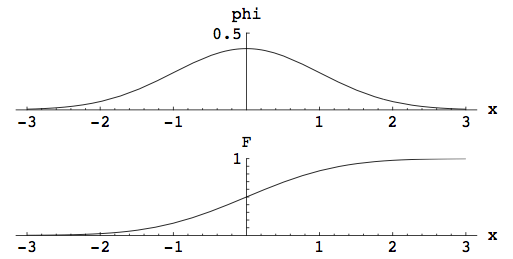
\includegraphics[width=8cm]{bilder/normalverteilung.png}
		Dichtefunktion (oben) und Verteilungsfunktion (unten) der Normalverteilung. 
   		\end{minipage} \\ \\
	$ 68\% $ der Werte liegen im Intervall $[ \mu - \sigma, \mu + \sigma]$, 
	$95\% $ in $[ \mu - 2\sigma, \mu + 2\sigma]$, 	
	$99.7\% $ in $[ \mu - 3\sigma, \mu + 3\sigma]$

	\subsubsection{Zentraler Grenzwertsatz }
      	$X_1, X_2, \ldots , X_n$ sind lauter identisch verteilte (nicht notwendig normalverteilt!)
      	unabh�ngige Zufallsvariablen mit demselben Erwartungswert $\mu$ und derselben Varianz $\sigma^2$.
      	\\ 
      	Dann hat die Summe ($S_n = \sum_{i=1}^n X_i$) den Erwartungswert $n \mu$ und die Varianz
      	$n \sigma^2$. \\
      	Die damit verbundene standardisierte ($E(X) = 0, var(X) = 1$) Variable $Z_n$ ist somit wie
      	folgt definiert: \\ $ Z_n = \dfrac{S_n - n \mu}{\sqrt{n} \sigma} = \dfrac{\overline{X} - \mu}{\sigma
      	/ \sqrt{n}}$
      	\\
      	F�r $\boldsymbol{n \to \infty}$ strebt die Verteilung von $Z_n$ gegen die
      	Standardnormalverteilung. \\
        

\newpage

 
\section{Informationstheorie }
\subsection{Informationsgehalt, Binary Unit, Entropie, Informationsrate}
Mathematisch gesehen kann man sagen, je \textbf{unwahrscheinlicher} das \textbf{Eintreten} eines \textbf{spezifischen
Ereignisses} ist, desto \textbf{gr�sser} ist dessen \textbf{Informationsgehalt}. \\

\begin{minipage}[c]{13cm}
	$$ I(x_i) = \log_{base} \frac{1}{P(x_i)} = - \log_{base} P(x_i) \qquad \qquad  R = r H (X)$$
	$$ H(X) = E[I(x_i)] = \sum\limits_{i=1}^m P(x_i) I(x_i) = - \sum\limits_{i=1}^m P(x_i)
	\log_2{P(x_i)} \qquad 0 \leq H(x) \leq \log_2(m)$$
	$$ H(X|Y)=- \sum\limits_{j=1}^{n} \sum\limits_{i=1}^{m} P(x_i,y_j)
	log_2(P(x_i|y_j))$$
	$$ H(X,Y)=- \sum\limits_{j=1}^{n} \sum\limits_{i=1}^{m}
	P(x_i,y_j)log_2(P(x_i,y_j)) =H(X)+HY|Y)=H(Y) + H(X|Y)$$
	$$I(X;Y)=I(Y;X)=H(X)+H(Y)-H(X,Y)=H(X)-H(X|Y)$$
	\textbf{Bin�re Entropie:}
	$$u(P(x_i))=-P(x_i) log_2(P(x_i))-(1-P(x_i) log_2(1-P(x_i)))$$
\end{minipage}
\begin{minipage}[c]{7cm}
	$I(x_i)$ Informationsgehalt, $[I(x_i)] = b$ \\\\
	$base = 2$ siehe nachfolgender Text\\\\
	$P(x_i)$ Auftretens-WSK eines Symbols \\\\
	$H(x_i)$ Entropie, $[H(x_i)] = $ b/Symbol \\\\
	$R$ Informationsrate, $[R]$ = b/s  \\\\
	$r$ Symbolrate, $[r]$ = Symbole/s 
%	$$
\end{minipage}
\vspace{0.2cm} \\
Der Informationsgehalt kann in folgenden Masseinheiten angegeben werden: \\
$$ [I(X)] = \begin{cases}
            	\text{bit (\emph{bi}nary uni\emph{t})}
            		& \text{falls } base=2. \\
            	\text{hartley oder decit}
            		& \text{falls } base=10. \\
            	\text{nat (\emph{na}tural uni\emph{t})}
            		& \text{falls } base=e
			\end{cases} $$

\textbf{Standartm�ssig} verwenden wir $base=2$, also bit oder gek�rzt \textbf{b}. Binary Unit ist
ein Mass f�r den Informationsgehalt und sollte nicht mit dem Term ``bit'' (Bin�res Zeichen) verwechselt
werden.

\subsection{DMS - Discrete Memoryless Source}
Eine Informations\textbf{quelle} ist ein Objekt welches \textbf{Ereignise}, welche zuf�llig aus einer
WSK-Dichtefunktion ausgew�hlt werden, \textbf{generiert}. \\
Eine diskrete Quelle hat einen endlichen \textbf{Satz an Symbolen}, welcher auch \textbf{Alphabet}
genannt wird. Die Elemente dieses Satzes nennt man \textbf{Symbole} oder \textbf{Zeichen}. \\
Wird ein Symbol unabh�ngig vom Vorherigen generiert, so handelt es sich um eine DMS (diskrete
ged�chtnisfreie Quelle). Eine solche wird mit folgenden Eigenschaften charakterisiert:
\begin{itemize}
  \item Liste der Symbole - Alphabet
  \item Auftretenswahrscheinlichkeiten dieser Symbole - WSK-Dichtefunktion
  \item Symbolrate
\end{itemize}


\subsection{DMC - Discrete Memoryless Channels}
\begin{minipage}{9.5cm}
	\begin{center}
		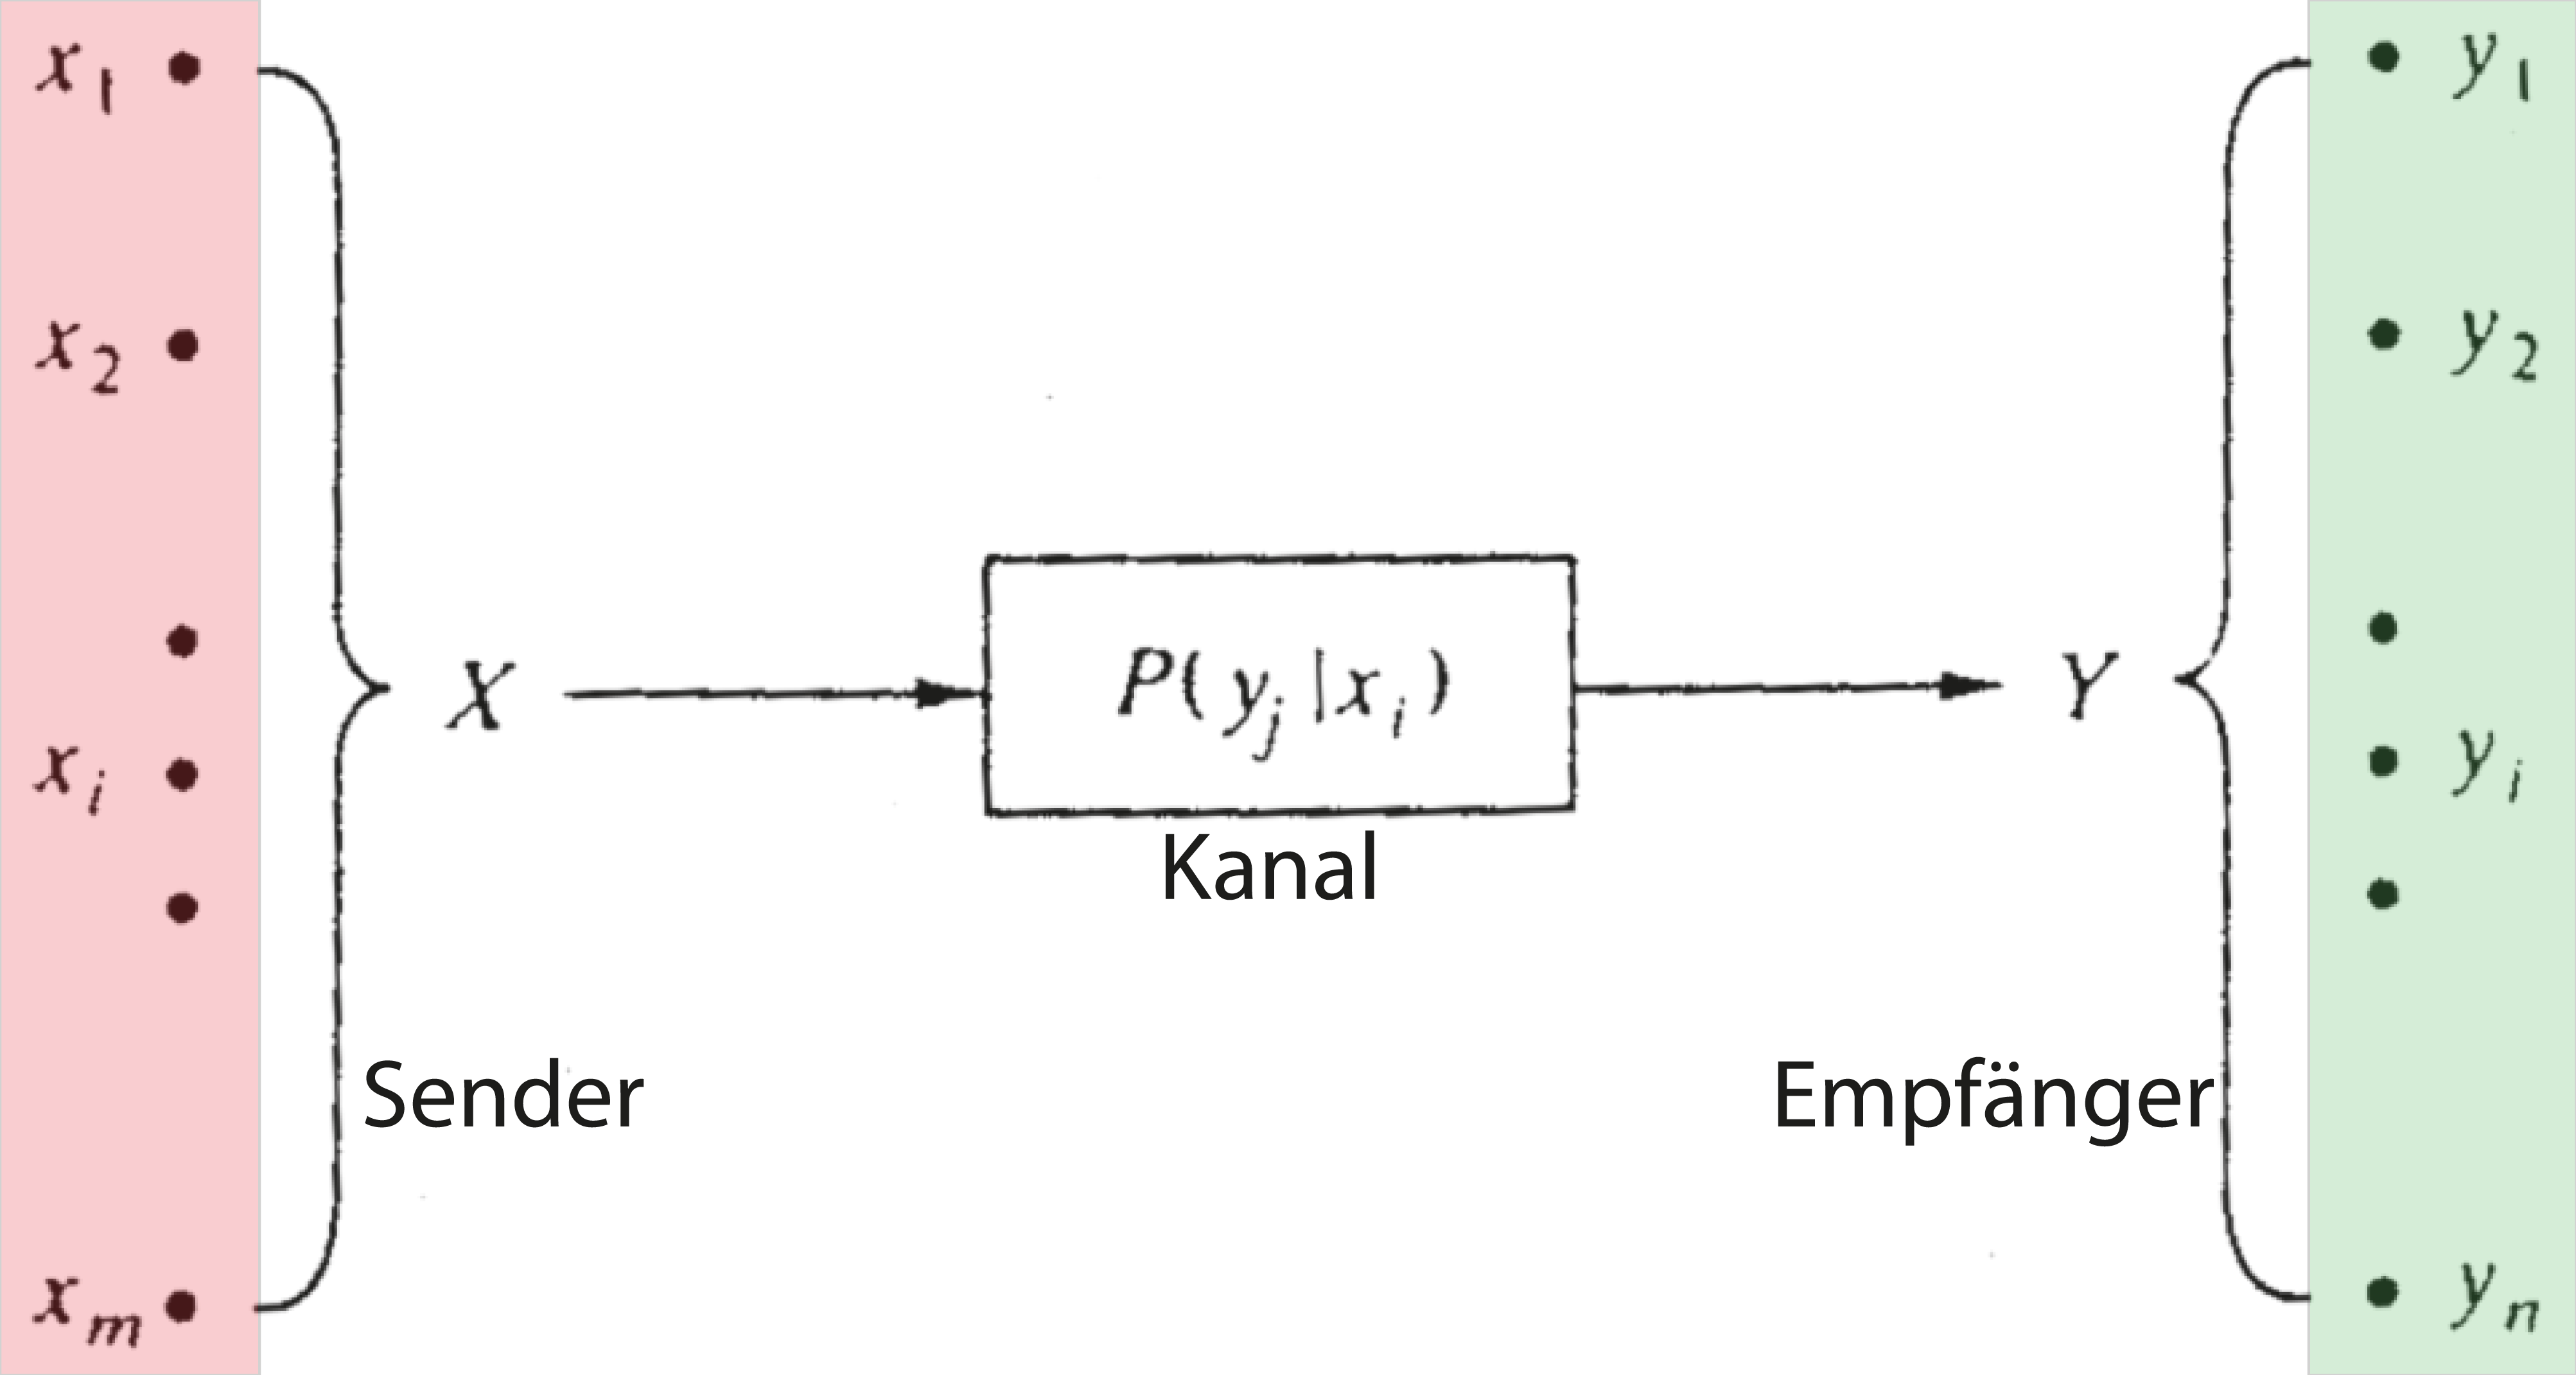
\includegraphics[width=8cm]{../NaT2/bilder/10_DMC.png}
	\end{center}
\end{minipage}
\begin{minipage}{8.5cm}
	Ein DMC (diskreter ged�chtnisfreier Kanal) ist ein statistisches Modell mit Eingang $X$ und
	Ausgang $Y$. \\ \\
	Er besitzt \textbf{$m$ Eing�nge} und \textbf{$n$ Ausg�nge}. \\ \\
	Alle Auftretenswahrscheinlichkeiten $P(x_i)$ der einzelnen Eingangs-Symbole werden als gegeben
	betrachtet. \\
	Jeder �bertragungspfad ist durch die Kanal-�bertragungs-Wahrscheinlichkeiten (channel transition
	probabilities) $P(y_j | x_i)$ definiert.
\end{minipage}

\subsubsection{Darstellung in Matritzenform}
\begin{minipage}{9cm}
	\textbf{Kanalmatrix}
	$$ [P(Y | X)] = \begin{bmatrix}
              P(y_1 | x_1) & P(y_2 | x_1) & \ldots & P(y_n | x_1) \\
              P(y_1 | x_2) & P(y_2 | x_2) & \ldots & P(y_n | x_2) \\
             \vdots & \vdots & \vdots & \vdots \\
              P(y_1 | x_m) & P(y_2 | x_m) & \ldots & P(y_n | x_m)
           \end{bmatrix}$$ \\
	$ [P(Y)] = [P(X)] \cdot [P(Y|X)]$ und $\sum\limits_{j=1}^n P(y_j | x_i) = 1 (\forall i)$
\end{minipage}
\begin{minipage}{9cm}
	\textbf{Verbundmatrix}
	$$ [P(Y,X)] = \begin{bmatrix}
              P(y_1, x_1) & P(y_2, x_1) & \ldots & P(y_n, x_1) \\
              P(y_1, x_2) & P(y_2, x_2) & \ldots & P(y_n, x_2) \\
             \vdots & \vdots & \vdots & \vdots \\
              P(y_1, x_m) & P(y_2, x_m) & \ldots & P(y_n, x_m)
           \end{bmatrix}$$
	$  [P(Y,X)] =  [P(X)]_d [P(Y|X)] $ \\
	Elemente auf der Diagonale sollten den gr�ssten Wert gegen�ber anderen Elementen auf der Zeile
	besitzen.
\end{minipage}

\subsubsection{Spezielle Kan�le}

\textbf{uniformly Dispersive} \\
\begin{minipage}{10cm}
Ein Kanal ist uniformly Dispersive, wenn ide WSK von einem Eingang zu den
Ausg�nge gleich wie bei den anderen Eing�ngen ist. z.B.:
\end{minipage}
\begin{minipage}{9cm}
	$$ [P(Y | X)] = \begin{bmatrix}
              \frac34 & \frac14 &  0 & 0 \\
              0 & \frac34 & \frac14 & 0 \\
              0 & 0 & \frac34 & \frac14 \\
              \frac14 &  0 & 0 &\frac34 \\
           \end{bmatrix}$$ \\
\end{minipage}        
           
\textbf{Verlustfreier(lossless) Kanal}\\
\begin{minipage}{14cm}
	Auf jeder Spalte der Kanalmatrix gibt es jeweils nur ein  Element $\neq 0$. \\

	$$ [P(Y | X)] = \begin{bmatrix}
              \frac34 & \frac14 & 0 & 0 & 0 \\
              0 & 0 & \frac13 & \frac23 & 0 \\
              0 & 0 & 0 & 0 & 1
           \end{bmatrix}$$ 
\end{minipage}
\begin{minipage}{4cm}
\begin{center}
	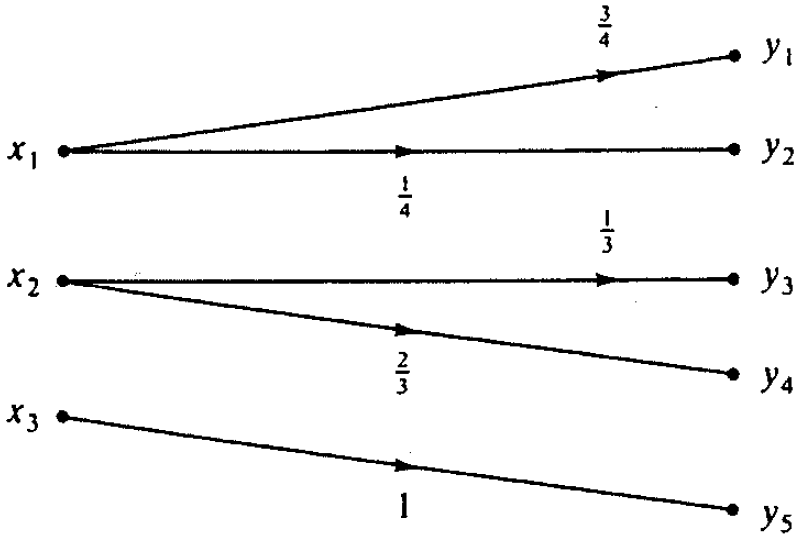
\includegraphics[height=3cm]{../NaT2/bilder/10_channels_lossless.png}
\end{center}
\end{minipage}

\textbf{Deterministischer (deterministic) Kanal} \\
\begin{minipage}{14cm}
	Auf jeder Zeile der Kanalmatrix gibt es jeweils nur ein  Element $\neq 0$, welches $1$ sein
	muss.

	$$ [P(Y | X)] = \begin{bmatrix}
           		1 & 0 & 0 \\
           		1 & 0 & 0 \\
           		0 & 1 & 0 \\
           		0 & 1 & 0 \\
           		0 & 0 & 1
           \end{bmatrix}$$
\end{minipage}
\begin{minipage}{4cm}
\begin{center}
	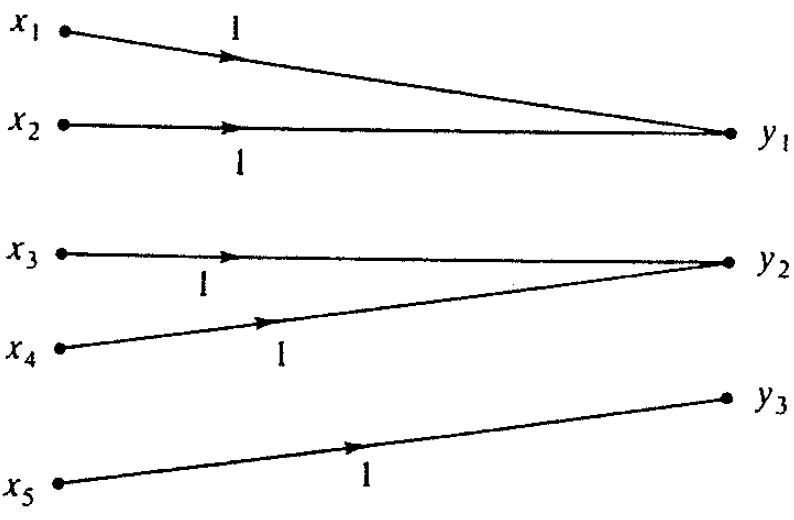
\includegraphics[height=3cm]{../NaT2/bilder/10_channels_deterministic.png}
\end{center}
\end{minipage}

\textbf{Rauschfreier (noiseless) Kanal} \\
\begin{minipage}{14cm}
	Die Kanalmatrix entspricht der Einheitsmatrix.

	$$ [P(Y | X)] = \begin{bmatrix}
           		1 & 0 & \ldots & 0\\
           		0 & 1 & \ldots & 0\\
           		\vdots & \vdots & \vdots & \vdots \\
           		0 & 0 & \ldots & 1\\
           \end{bmatrix} = I$$ \\
\end{minipage}
\begin{minipage}{4cm}
\begin{center}
	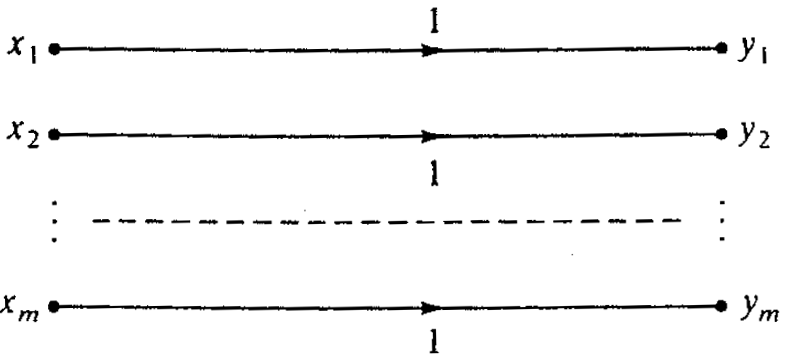
\includegraphics[width=4.5cm]{../NaT2/bilder/10_channels_noiseless.png}
\end{center}
\end{minipage}

\textbf{BSC- Bin�rer Symmetrischer (binary symmetrical) Kanal} \\
\begin{minipage}{14cm}

	$$ [P(Y | X)] = \begin{bmatrix}
           		1-p & p \\
           		p & 1-p
           \end{bmatrix} $$
\end{minipage}
\begin{minipage}{4cm}
\begin{center}
	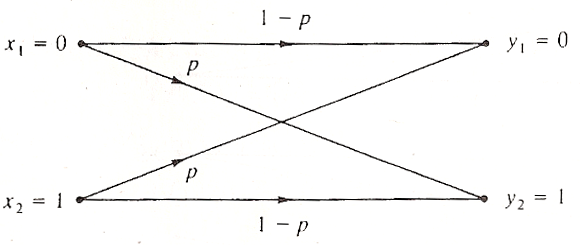
\includegraphics[width=4.5cm]{../NaT2/bilder/10_channels_binarysymmetrical.png}
\end{center}
\end{minipage}


\textbf{BEC - Bin�rer Ausl�schungs (binary erasure) Kanal} \\
\begin{minipage}{14cm}

	$$ P_{Y | X}(0|1) =  P_{Y | X}(1|0) = 0 $$
	$$ P_{Y | X}(0|0) =  P_{Y | X}(1|1) = 1-\delta $$
	$$ P_{Y | X}(\delta|0) =  P_{Y | X}(\delta|1) = \delta $$
\end{minipage}
\begin{minipage}{4cm}
\begin{center}
	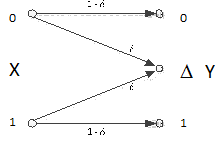
\includegraphics[width=4.5cm]{./bilder/10_channels_binaryErasure.png}
\end{center}
\end{minipage}

\textbf{Uniformly dispersive Canal} \\
Wenn die Wahrscheinlich (in einem Vektor angeorgnet und sortiert) gleich sind.
\\
z.B. $$
[\frac{1}{2},\frac{1}{4},\frac{1}{4}]=[\frac{1}{2},\frac{1}{4},\frac{1}{4}]\neq
[\frac{1}{2},\frac{1}{2}]$$


\subsection{Kanalkapazit�t}
\begin{minipage}[c]{8cm}
	$$ C_s = \max\limits_{\{ P(x_i) \}}{I (X; Y)} 
	 = \max\limits_{\{ P(x_i)\}}{H(X)- H(X|Y)} $$
	$$ = \max\limits_{\{ P(x_i)\}}{H(Y)- H(Y|X)} $$ 
	$$ C = r C_s $$
\end{minipage}
\begin{minipage}[c]{10cm}
	$C_s$ Kanalkapazit�t pro Symbol, $[C_s]$ = b/Symbol \\
	$C$ Kanalkapazit�t pro Sekunde, $[C]$ = b/s \\
	$r$ Symbolrate, $[r]$ = Symbol/s
%	$$
\end{minipage}\\
Wenn Informationsrate  $R < C \Rightarrow \epsilon = Fehlerrate = 0$  ist
m�glich


\subsection{AWGN-Channel}
AWGN = Additiv White Gausian Noise. $y(t)=x(t)+w(t)$ $w(t)$: white noise with
spectral density $\frac{N_0}2$

\subsubsection{Kanalkapazit�tien spezieller Kan�le}

	\renewcommand{\arraystretch}{2}
	\begin{tabular}{| p{3.5cm} | p{7.5cm} | p{6.5cm} |}
		\hline
    		\textbf{Verlustfrei}
    			& $ I(X; Y) = H(X) $
    			& $ C_s = \max\limits_{\{ P(x_i) \}}{H (X)} = \log_2 m $ \\
		\hline
    		\textbf{Deterministisch}
    			& $ I(X; Y) = H(Y) $
    			& $ C_s = \max\limits_{\{ P(x_i) \}}{H (Y)} = \log_2 n $ \\
		\hline
    		\textbf{Rauschfrei}
    			& $ I(X; Y) = H(Y) = H(X)$
    			& $ C_s = \log_2 n = \log_2 m$ \\
		\hline
    		\textbf{Bin�r Symmetrisch}
    			& $ I(X; Y) = H(Y) + p \log_2 p + (1-p) \log_2 (1-p)$
    			& $ C_s = 1 + p \log_2 p + (1-p) \log_2 (1-p)$ \\
		\hline
    		\textbf{Bin�r Symmetrisch}
    			& & $ C_s = 1 + \delta $ \\
		\hline
    		\textbf{AWGN}
    			& $ C = 2 B C_s = B \log_2 (1 + \frac{S}{N})= B \log_2 (1 +
    			\frac{P}{N_0 B})$ & $ C_s = \max{I(X; Y) = \frac{1}{2} \log_2 (1 +
    			\frac{S}{N})}$ \\
		\hline
 	\end{tabular}
	\renewcommand{\arraystretch}{1} \\ \\
Wobei $B$ der Bandbreite des Kanals entspricht.

\subsection{Water filling}
\begin{minipage}{12cm}
Ziel ist es die Leistung auf die Frequenzen zu verteilen auf denen das Rauschen
m�glichst klein ist. \\
 $$C=\int log_2(1+\frac{P(t) |H(t)|^2}{N_0}) $$
 $$P(t)= \frac 1\lambda - \frac{N_0}{|H(f)|^2}; N_0= \eta B$$
 $$ \lambda: \int \limits_0^B max(0, \frac 1\lambda - \frac{N_0}{|H(f)|^2})=P$$
\end{minipage}
\begin{minipage}{6cm}
	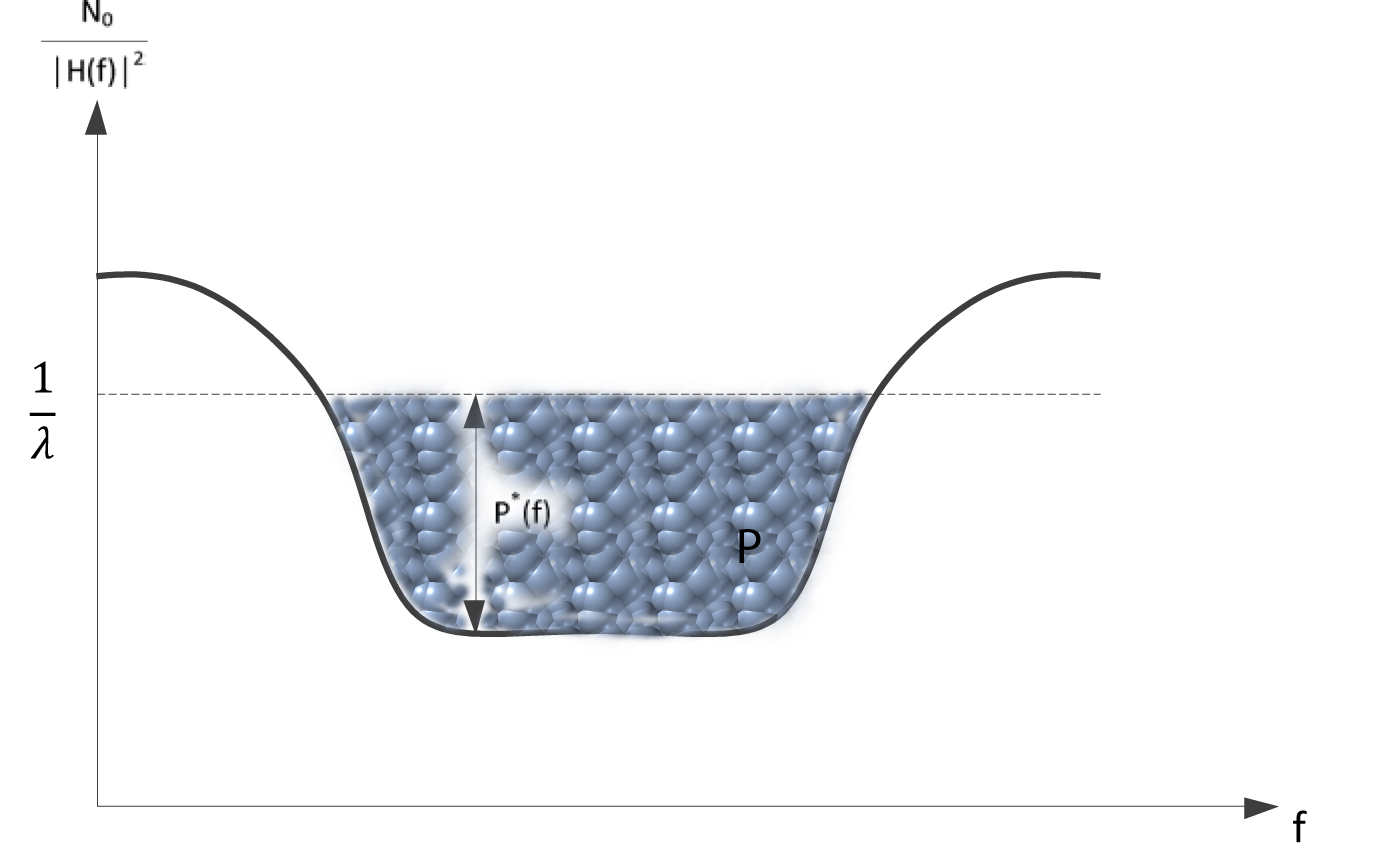
\includegraphics[width=6cm]{./bilder/Waterfilling.png}

\end{minipage}

\newpage

\section{Wave Propagation}
\subsection{Luftkanal }
\begin{tabular}{ll}
\parbox{8cm}{
    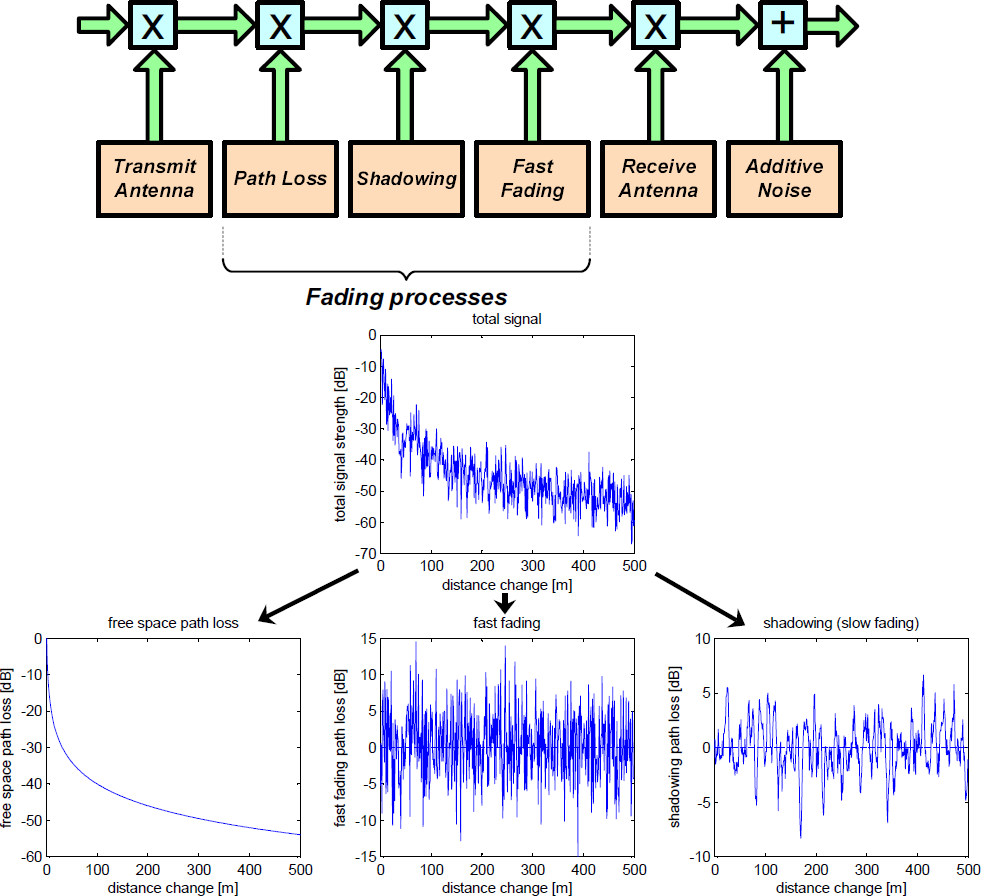
\includegraphics[width=7cm]{../MobKom2/bilder/antennas-noisetypes.png}}
& \parbox{10cm}{
    Rauschtypen:
    \begin{liste}
        \item Additives Rauschen
        \begin{liste}
            \item Thermisches, Flicker/Funkel/$\frac{1}{f}$, Shot Rauschen
            \item Atmosph�rischer Einfluss, Kosmische Strahlung, St�rungen von
            anderen el. Quellen
        \end{liste}
        \item Multiplikatives Rauschen
        \begin{liste}
            \item Richtungsabh�ngigkeit der Antennen
            \item Reflektionen
            \item Absorptionen
            \item Streuungen (Scattering)
            \item Beugung (Diffraction)
            \item Brechnung (Refraction)
        \end{liste}
    \end{liste}}
\end{tabular}
\subsection{Einf�hrung }
\begin{liste}
    \item Pfadverlust in Kabel: Linear zur Distanz; in der Luft: Logarithmisch zur Distanz
    \item Nah- \& Fernfeld: Grenze bei $R = \frac{2L^2}{\lambda}$
    \item Impedanz in der Luft: 
    $Z=\frac{|E|}{|H|}=\sqrt{\frac{\mu_0}{\varepsilon_0}}=120\pi \,\Omega= 377\,\Omega$
\end{liste}
\subsection{Rauschen}
\subsubsection{Weisses Rauschen}
\begin{center}
	\begin{minipage}{8cm}
		$S_{XX}(\omega) = \dfrac{\eta}{2} \qquad R_{XX}(\tau) = \dfrac{\eta}{2} \cdot \delta(\tau)$ \\ \\
		Beispiel: therm. Rauschen von Widerst�nden \\
		\textbf{Nimmt} in der Praxis im \textbf{Tera-Hz Bereich ab}!
  	\end{minipage}
	\begin{minipage}{10cm}
		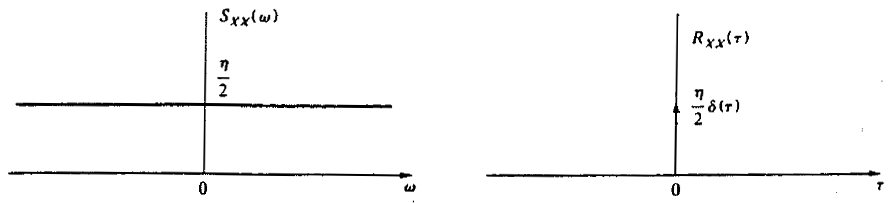
\includegraphics[width=9cm]{../NaT2/bilder/07_weisses_rauschen.png}
  	\end{minipage}
\end{center}

\subsubsection{Bandbeschr�nktes Rauschen}
\begin{center}
	\begin{minipage}{8cm}
		$S_{XX}(\omega) = \begin{cases}
                      \dfrac{\eta}{2} & |\omega| \leq \omega_B \\
                      0 & |\omega| > \omega_B
                      \end{cases} \\ \\
		R_{XX}(\tau) =  \frac{1}{2\pi} \int\limits_{-\omega_{b}}^{+\omega_{b}}
                                           \frac{\eta}{2}  \cdot e^{j\omega\tau}\; d\tau
                      = \frac{\eta\omega_{B}}{2\pi} \frac{\sin(\omega_{B}\tau)}{\omega_{B}\tau}$
  	\end{minipage}
	\begin{minipage}{10cm}
		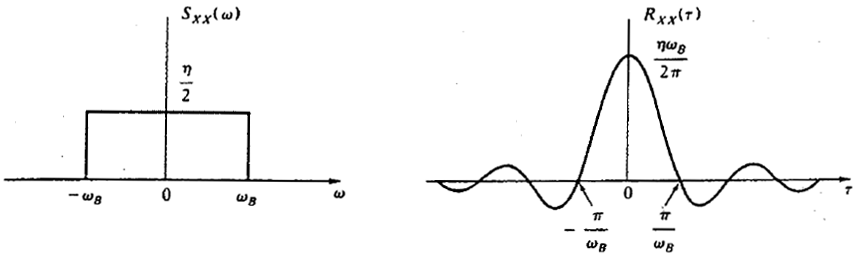
\includegraphics[width=9cm]{../NaT2/bilder/07_bandlimited_whitenoise.png}
  	\end{minipage}
\end{center}

\subsubsection{SNR}
Wegen dem Eigenrauschen $\text{N}_{\text{out,total}}$ des Verst�rkers ist das
$\text{SNR}$ am Ausgang des Verst�rkers kleiner (also schlechter) als dasjenige am Eingang. Diese Differenz ist durch die noise figure NF (in dB)
oder den noise factor $F$ (linear) gegeben.
\vspace{0.1cm}\\
$ \boxed{F = \dfrac{\text{SNR}_{\text{in}}}{\text{SNR}_{\text{out}}} =
\dfrac{\text{N}_{\text{out,total}}}{\text{N}_{\text{out,source}}}=
\dfrac{\text{N}_{\text{out,total}}}{\text{G}\cdot \text{N}_{\text{in}}}}
\qquad \Longleftrightarrow \qquad \boxed{\text{NF} = 10 \cdot \logd (F) =
\text{SNR}_{in.dB} - \text{SNR}_{out.dB} =
\text{N}_{\text{out,total,dB}}-(\text{G}_{dB}+ \text{N}_{\text{in,dB}})}$
\vspace{0.1cm}\\
$ N_{in} = k T B \qquad \text{mit } k = 1.38 \cdot
10^{-23} \qquad (k T_0)_{dB} |_{T_0 = 290K} = -174 \text{dBm/Hz} \qquad
N_{in,dB} = (k T_0)_{dB} + 10 \logd (B)$ \\
\vspace{0.1cm}
Die Bandbreite $B$ des Rauschen
$N_{in}$ ist durch das schmalbandigste Filter in einer Kaskade definiert.
\vspace{0.2cm}
Ver�nderung der SNR bzgl. Rauschen: $\qquad \text{SNR}_{out.dB} <
\text{SNR}_{in.dB} \qquad \text{SNR}_{out.dB} = \text{SNR}_{in.dB} - \text{NF}
= (S_{in.dB} - N_{in.dB}) - \text{NF}$

\begin{tabular}{ll}
\parbox{9cm}{
    \textbf{Kaskadierte Bl�cke} \\
    $$G = G_1 \cdot G_2 \cdot \cdot \cdot G_k \qquad G_{dB} = G_{1.dB} + G_{2.dB} + \cdot \cdot
    \cdot + G_{k.dB}$$
    $$F=F_1+\dfrac{F_2-1}{G_1}+ \dfrac{F_3-1}{G_1G_2}+\ldots
       + \dfrac{F_K-1}{G_1G_2\cdots G_{K-1}}$$
       $$\text{Unendliche Kaskade: }F_{\infty} = F + \dfrac{F-1}{G-1} =
       \dfrac{G \cdot F-1}{G-1}$$ F�r passive Komponenten gilt: $F =
       \frac{1}{G_{passive}}; G = G_{passive}$ }
& \parbox{9cm}{
        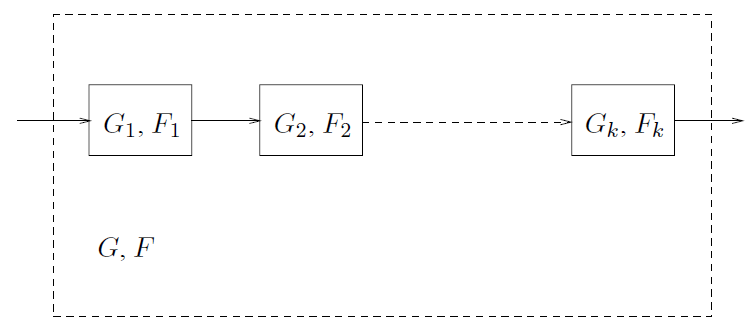
\includegraphics[width=9cm]{../MobKom1/bilder/components_amplifier_noise_cascade.png}
        }\\
\end{tabular}\\

Grunds�tzlich \textbf{dominiert} das \textbf{erste Element} einer Kaskade die noise figure NF. Ist dessen noise factor
$F_1$ klein und die Verst�rkung $G_1$ gross, so wird der gesamte noise factor $F$ klein. Dies sind
u.a. Eigenschaften von LNA-Verst�rkern.\\

\begin{tabular}{ll}
\parbox{12cm}{
    \textbf{Funkelrauschen - flicker noise} \\
    Bei tieferen Frequenzen $f$ domitiert das Funkel- oder auch 1/f-Rauschen gegen�ber dem
    thermischen Rauschen. \\ \\
    \parbox{8cm}{
    \begin{tabular}{|l|l|}\hline
    Element & corner frequency $f_c$ \\ \hline \hline
    Si-bipolar transistors & 100\,Hz to 1\,kHz \\ \hline
    Si-MOSFET              & 100\,Hz to 1\,MHz \\ \hline
    GaAs-MESFET            & 1\,MHz to 50\,MHz \\ \hline
    \end{tabular}
	}
    \parbox{3cm}{
    $F=F_0 \cdot \left(\frac{f_c}{f}+ 1\right)$
    }
 %\includegraphics[height=2.5cm]{../MobKom1/bilder/components_amplifier_noise_flicker_table.png}
    }
& \parbox{6cm}{
        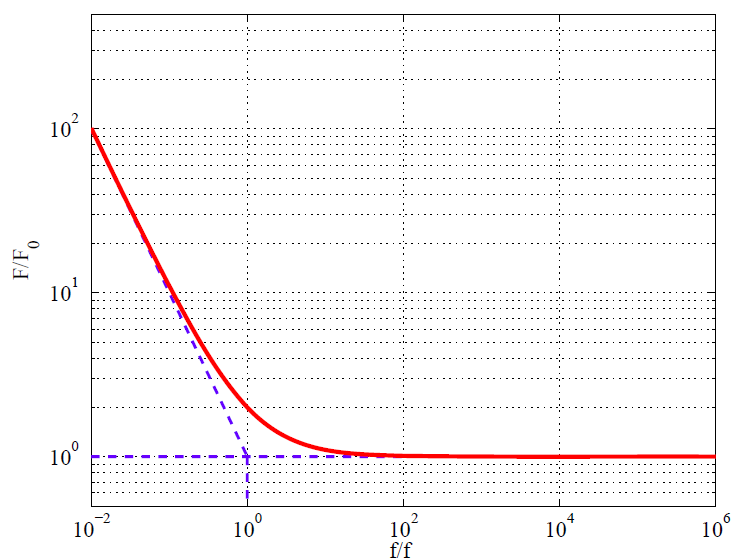
\includegraphics[height=4cm]{../MobKom1/bilder/components_amplifier_noise_flicker.png}
        }\\
\end{tabular}

\subsection{Luftlose �bertragung}
\begin{tabular}{|l|c|}
\hline
\textbf{Modell}
    & \textbf{Abbildung}\\
\hline
\hline
\parbox{10cm}{
    \textbf{Free-space propagation} \\
    \begin{minipage}{6cm}
	    \begin{liste}
	        \item Keine Reflektionen
	        \item Keine Hindernisse
	        \item Kein Multipath
	        \item Zu optimistisch/idealisiert
	    \end{liste}        
    \end{minipage}
    \begin{minipage}{3cm}
        $$ P_R= \frac{P_TG_T}{4\pi r^2} A_R $$
        $$ \frac{P_R}{P_T} = G_TG_R \left(\frac{\lambda}{4\pi r}\right)^2  $$
    \end{minipage}

    $$L=\frac{P_TG_TG_R}{P_R} = \left(\frac{4\pi r}{\lambda}\right)^2 =
    \left(\frac{4\pi rf}{c}\right)^2$$ 
    $$L\,\text{[dB]} = -147.6 + 20\log r + 20\log f$$ }
    & \parbox{3cm}{
        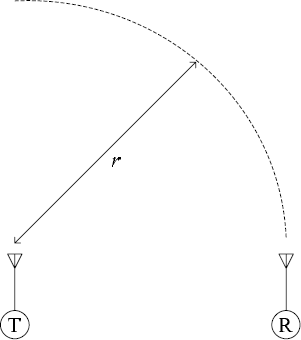
\includegraphics[width=3cm]{../MobKom2/bilder/propagation-freespace.png}
        } \\
\hline
\parbox{10cm}{
    \textbf{Open-field/Plane-earth propagation} \\
    \begin{liste}
        \item Keine Hindernisse    
        \item Einfache Reflektion am Boden (zwei Pfade)
        \item Zweiter Pfad kann konstruktiv oder destruktiv sein
    \end{liste}
    $$L= 4\frac{\pi r}{\lambda}^2
       \sin^{-2} \frac{2\pi h_bh_m}{\lambda r} \quad \text{f�r } r <
       r_x=\frac{4h_bh_m}{\lambda}$$ 
    $$L= \frac{r^4}{h_b^2h_m^2} \quad \text{f�r } r > r_x$$
    }
    & \parbox{5cm}{
        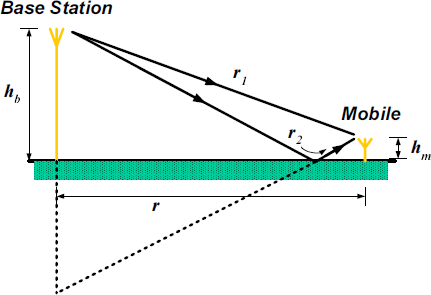
\includegraphics[width=5cm]{../MobKom2/bilder/propagation-openfield.png}
        } \\
\hline
\end{tabular}\\
\begin{tabular}{|l|c|}
\hline
\parbox{10cm}{
    \textbf{Simulation (rechts)}:\\
    $h_b=20\,$m, $h_m=1.5\,$m, $f=1\,$GHz \\
    
    \textbf{Weitere Modelle}\\
    Exponent $n$ der Entfernung $r^n$ haupts�chlich massgebend f�r Modell.
    Weitere M�glichkeiten:
    
    \begin{tabular}{|l|r|}
	\hline
	environment & path-loss exponent $n$      \\ \hline \hline
	free space                     & 2        \\ \hline
	open field (long distance)     & 4        \\ \hline
	cellular radio, urban area     & 2.7--4   \\ \hline
	shadowed urban cellular radio  & 5--6     \\ \hline
	in building, line-of-sight     & 1.6--1.8 \\ \hline
	in building, obstructed        & 4--6     \\ \hline
	\end{tabular}
    }
    & \parbox{8cm}{
    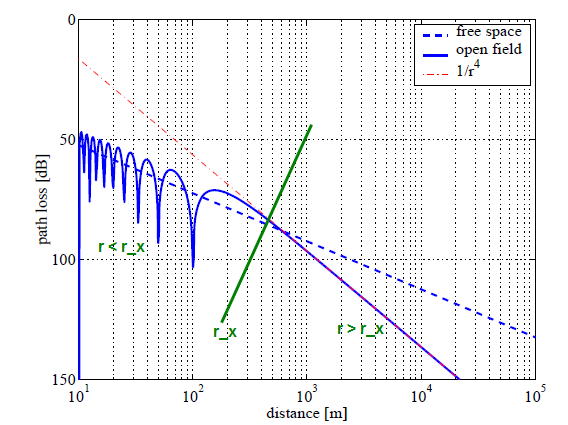
\includegraphics[width=8cm]{../MobKom2/bilder/propagation-simulation.png}
    } \\
\hline
\parbox{10cm}{
    \textbf{Okumura-Hata}:\\
    \begin{liste}
        \item Transmit frequency: f = 150...1500 MHz
        \item Height of base station antenna: $h_{BS}$ = 30...200 m
        \item Height of mobile station antenna: $h_{MS}$ = 1...10 m
        \item Distance: 1...20 km
    \end{liste}
    Path-Loss for urban enviroment:\\
    $L_{Hu}[dB] = 69.55+26.16 \logd( \frac{f}{MHz})- 13.82
    \logd(\frac{h_{BS}}{m})  - a(h_{MS}) + (44.9-6.55 \logd(\frac{h_{BS}}{m})) 
    \logd(\frac{d}{km}) $ \\
    } 
    & 
\parbox{8cm}{
  \textbf{Korrekturtur terme}:\\
    \begin{liste}
    	\item small and medium sized cities: \\
    	$a(h_{MS})=(1.1 \logd \frac{f}{MHz}- 0.7) \frac{h_{MS}}{m} - (1.56\logd 
    	(\frac{f}{MHz})-0.8)$
    	\item Metropolises:\\
    	$a(h_{MS})=\{^{(8.29 [\logd(1.54 \frac{h_{MS}}{m}) ]^2- 1.1) f\leq 200 MHz}
    	_{(3.2 [\logd(11.75 \frac{h_{MS}}{m}) ]^2- 4.97)  f\geq 400 MHz}$
    	\item sub-Urban: \\
    	$L_{Hs}[dB]=L_{Hu}-2 [\logd(\frac f{28MHz})]^2 -5.4$
    	\item rural areas:\\
    	$L_{Hr}[dB]= L_{Hu} - 4.78[\logd(\frac f{MHz})]^2 + 18.33 \logd(\frac
    	f{MHz}) - 40.94$
    \end{liste}
     } \\
\hline
\hline 
\parbox{10cm}{
    \textbf{Beugung (Diffraction)}:\\
    \begin{liste}
        \item Weitere Verluste durch Beugung
        \item Beugungsparameter: $v=h\sqrt{\dfrac{2(d_1+d_2)}{\lambda d_1d_2}}$
        \item Zus�tzlicher (zum Modell dazu) Pfadverlust: \\
        $L \approx 20\log (\sqrt 2\pi v) \approx 20\log \frac v{0.225} \quad
        v>1$
    \end{liste}
    \center{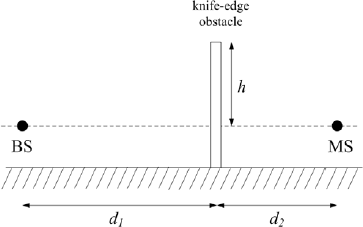
\includegraphics[width=5cm]{../MobKom2/bilder/propagation-diffraction.png}}
    }
    & \parbox{7cm}{
    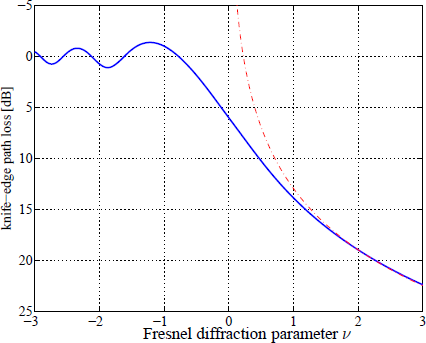
\includegraphics[width=7cm]{../MobKom2/bilder/propagation-fresnel-diffraction-parameter.png} } \\
\hline
\end{tabular}

\begin{tabular}{ll}
\parbox{11cm}{
	\subsection{Link Budget}
	\begin{liste}
	    \item Summierung aller (logarithmischen) Verluste und Gewinne vom Sender
	    zum Empf�nger
	    \item Noise power density (Rauschleistung) $N_0 = -174\text{dBm}$ (pro Hz)
	    \item Empf�nger- \& Sendergewinn ($G_T, G_R$) in DBi
	    \item Bsp: $P=N_0+10 \logd B+\text{NF}+\text{SNR}+L-G_T-G_R$
	\end{liste}

	\subsection{Shadowing (Slow Fading)}
	\begin{liste}
	    \item Tritt bei langsamen Bewegungen auf
	    \item Leichtes Entzerren, da hohe Korrelation
	    \item Normalverteilter Pfadverlust
	\end{liste}
    }
& \parbox{7cm}{
    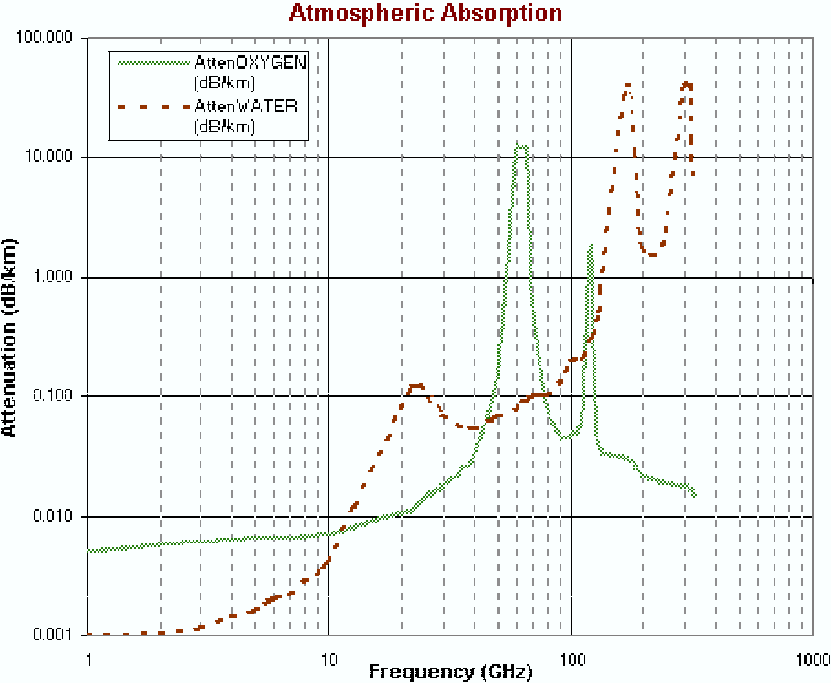
\includegraphics[width=7cm]{../MobKom2/bilder/propagation-atmospheric-absorption.png}}
\end{tabular}

\subsection{Fast Fading}
\begin{tabular}{|lll|}
\hline
\parbox{7cm}{
    \textbf{Non-line-of-sight (NLOS)} \\
    \begin{liste}
        \item Geh�rt zu flat fading (frequency non-selective)
        \item Rayleigh Verteilung $p(r) = \frac r{\sigma^2}
        e^{-\frac{r^2}{2\sigma^2}}$
    \end{liste}
    }
    & \parbox{5cm}{
        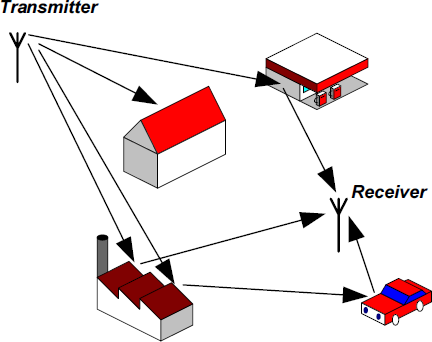
\includegraphics[width=5cm]{../MobKom2/bilder/propagation-nlos.png}
        } 
    &
    \multirow{2}{*}{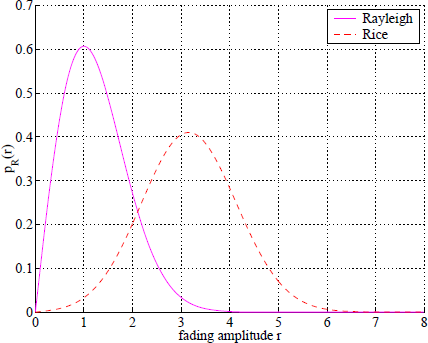
\includegraphics[width=5.5cm]{../MobKom2/bilder/propagation-fading-pdf.png}}
    \\
\parbox{7cm}{
    \textbf{Line-of-sight (LOS)} \\
    \begin{liste}
        \item Geh�rt zu flat fading (frequency non-selective)
        \item Rayleigh Verteilung $p(r) = \frac r{\sigma^2}
        e^{-\frac{r^2}{2\sigma^2}}$
    \end{liste}
    }
    & \parbox{5cm}{
        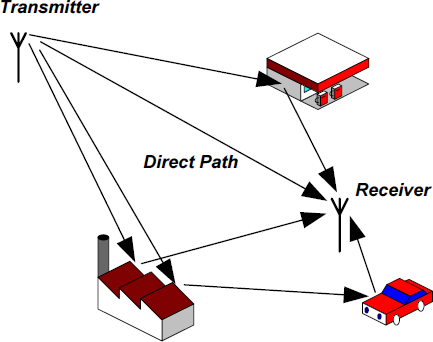
\includegraphics[width=5cm]{../MobKom2/bilder/propagation-los.png}
        } 
    & \\
\hline
\parbox{7cm}{
	    \textbf{Frequency selective fading (multipath)}
	    \begin{liste}
            \item {\em Mean delay}: $\tau_0=\frac 1{P_T}\sum\limits_k P_k
            \tau_k$
            \item {\em RMS delay spread}:\\
            $\tau_{\text{RMS}}=\sqrt{\frac{1}{P_T}}\sum\limits_k P_k
            (\tau_k-\tau_0)^2$
            \item Total power:
            $P_T=\sum\limits_k P_k$
        \end{liste}
    } 
    & \parbox{5cm}{
        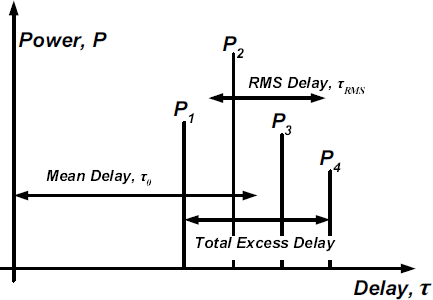
\includegraphics[width=5cm]{../MobKom2/bilder/propagation-frequency-selective-power-delay.png} 
        } 
    & \parbox{5cm}{ 
        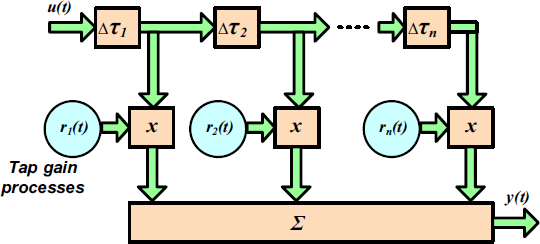
\includegraphics[width=5.5cm]{../MobKom2/bilder/propagation-frequency-selective-model.png} 
        } \\
\hline
\end{tabular}

\subsection{Beziehungen zwischen Fading Parameter}
\begin{liste}
    \item $T_c \propto  \frac 1{f_m}$ \qquad $T_c$ = Koh�renzzeit, $f_m$ =
    Dopplerverschiebung (spread)
    \item $B_c \propto \frac 1{\tau}$ \qquad $B_c$ = Koh�renzbandbreite, $\tau$
    = Zeitverbreiterung (broadeing)
    \item $B_c$, $T_c$ unabh�ngig
\end{liste}

\newpage

\section{Kanalzugriff und Modulation }
\subsection{Kanalzugriff}
	Den Kanalzugriff muss nur f�r Systeme mit mehreren unterschidlichen Sender bzw.
	Empf�ngern geregelt werden. Folgende M�glichkeiten bestehen:\\

\subsection{FDMA - Frequency Division Multiple Access - Frequenz-Multiplexing} 
Prinzip:\\Jeder Benutzer sendet auf einer zugewiesenen Frequenz mit einer definierten Bandbreite.\\
		Einsatzort:\\FM, aber auch GSM im Up-, wie auch im Downlink-Band (siehe
		Bild)\\
\subsection{TDMA - Time Division Multiple Access - Zeit-Multiplexing}


\begin{tabular}{ll}
\parbox{11cm}{
		Prinzip:\\Jeder Benutzer bekommt einen bestimmten Zeitschlitz, um in
		diesem Pakete senden zu k�nnen. Nach einer gewissen Zeit (Frame) wiederholt sich das
		ganze\\
		Einsatzort:\\zB. GSM: In einem Frame von 4.615ms hat es jeweils 8
		Teilnehmern (siehe Bild).}
    & \parbox{9cm}{
        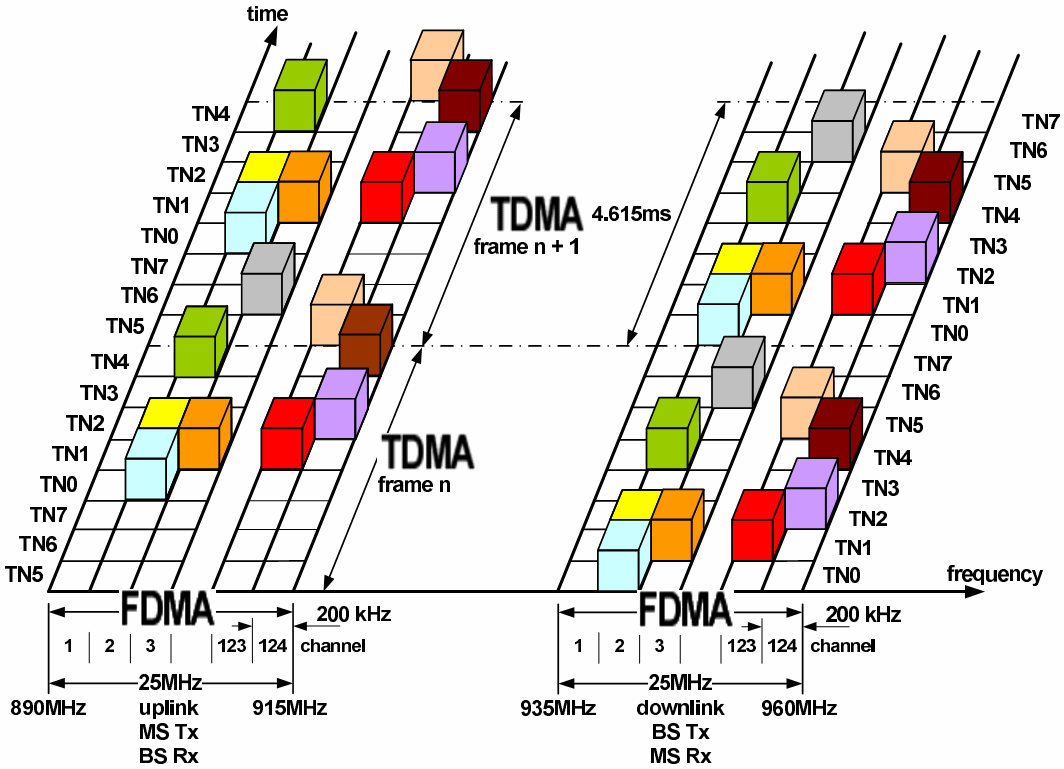
\includegraphics[width=6cm]{bilder/modulation_TDMA.png}
        } \\
\parbox{11cm}{
		Speziell: ALOHA\\
		F�r die Zuordnung der Zeitschlitze f�r einen neuen Teilnehmer meldet sich
		dieser zuerst bei der Basisstation. Dabei kann es zu Kollisionen mit anderen
		Teilnehmern kommen. Erneutes Melden bei der Basisstation erfolgt beim
		ALOHA-Prinzip erfolgt nach einer zuf�llige Zeitdauer, womit die erneute
		Kollision vermieden wird.} 
	& \parbox{9cm}{
	    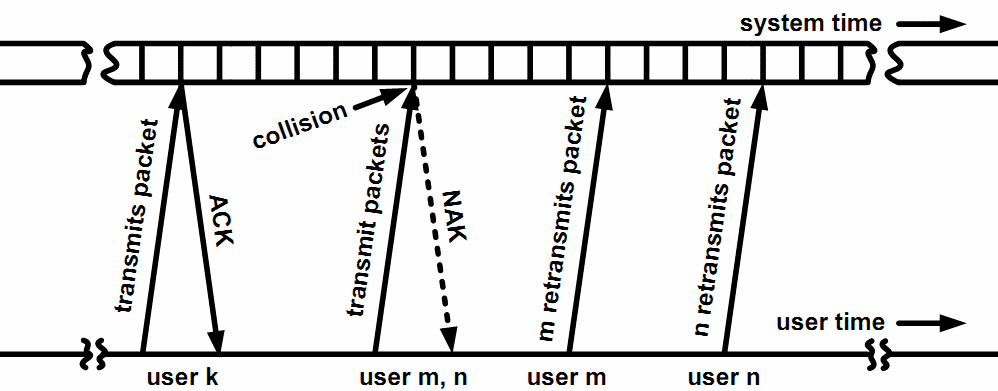
\includegraphics[width=6cm]{bilder/modulation_aloha.png}
	    }
\end{tabular}

\subsection{CDMA - Code Division Multiple Access - Code Multiplexing}
 
Prinzip:\\
Die Tr�gerfrequenzen werden mit Hilfe eines Codes zeitlich variiert. Durch eine
Korrelation mit demselben Codes kann man die richtigen Daten auch bei
�berlagerungen wieder herausfiltern. Deshalb k�nnen viele Sender bzw.
Empf�nger auf demselben Frequenzband arbeiten. CDMA brauch jedoch durch das
Frequenzhopping auch mehr Bandbreite.\\
Vorteil/Nachteile:\\
+ \textbf{Privacy: }Die Daten sind nur f�r die Empf�nger mit den richtigen Codes
sichtbar.\\
+ \textbf{Fading immunity: }Sicher gegen Frequenzl�cher (da CDMA eine grosse
Bandbreite benutzt).\\
+ \textbf{Jamming resistans: }St�rsicher gegen schmalbandige St�rsignale. \\
+ \textbf{Low spectral densy: } Signal kann sogar unterhalb des termischen
Rauschens sein\\
+ \textbf{Soft Handover: } Mit CDMA ist es m�glich einen Antennenwechsel
praktisch ohne Unterbruch zu machen, da nur der Code gewechselt wird und
keine Frequenzen.\\
+ Bei wenigen Teilnehmern sehr gute SNR\\
+ Gut f�r unkoordinierte Teilnehmer (da keine Absprachen bez�glich
Zeitschlitz, Kanalfrequenz, etc. n�tig sind).\\
- \textbf{Near-Far Problem: }Schlechtes Near-Far-Verhalten
(wenn ein starker (naher) Teilnehmer einen schwachen (fernen) unterdr�ckt). \\
- \textbf{komplexity: } Viel komplexerer Empfang. Man muss korrelieren, den
Dopppler Shift ausgleichen, etc. Synchronisiation sehr schwer.\\

% TODO: more about m-sequence
\textbf{more about m-sequencen}\\\\
% TODO: more about spreadingn Gain
\textbf{Spreadingn Gain}\\
$G=10 \log_{10}(\frac{SNR_{out}}{SNR_{in}})= 10
\log_{10}(\frac{B_{SS}}{B_d}=\frac{nach Spreading}{original})=10
\log_{10}(\frac{T_d}{T_c=ChipTime})$

\subsubsection{Korrelation}
	\begin{minipage}{6cm}
    	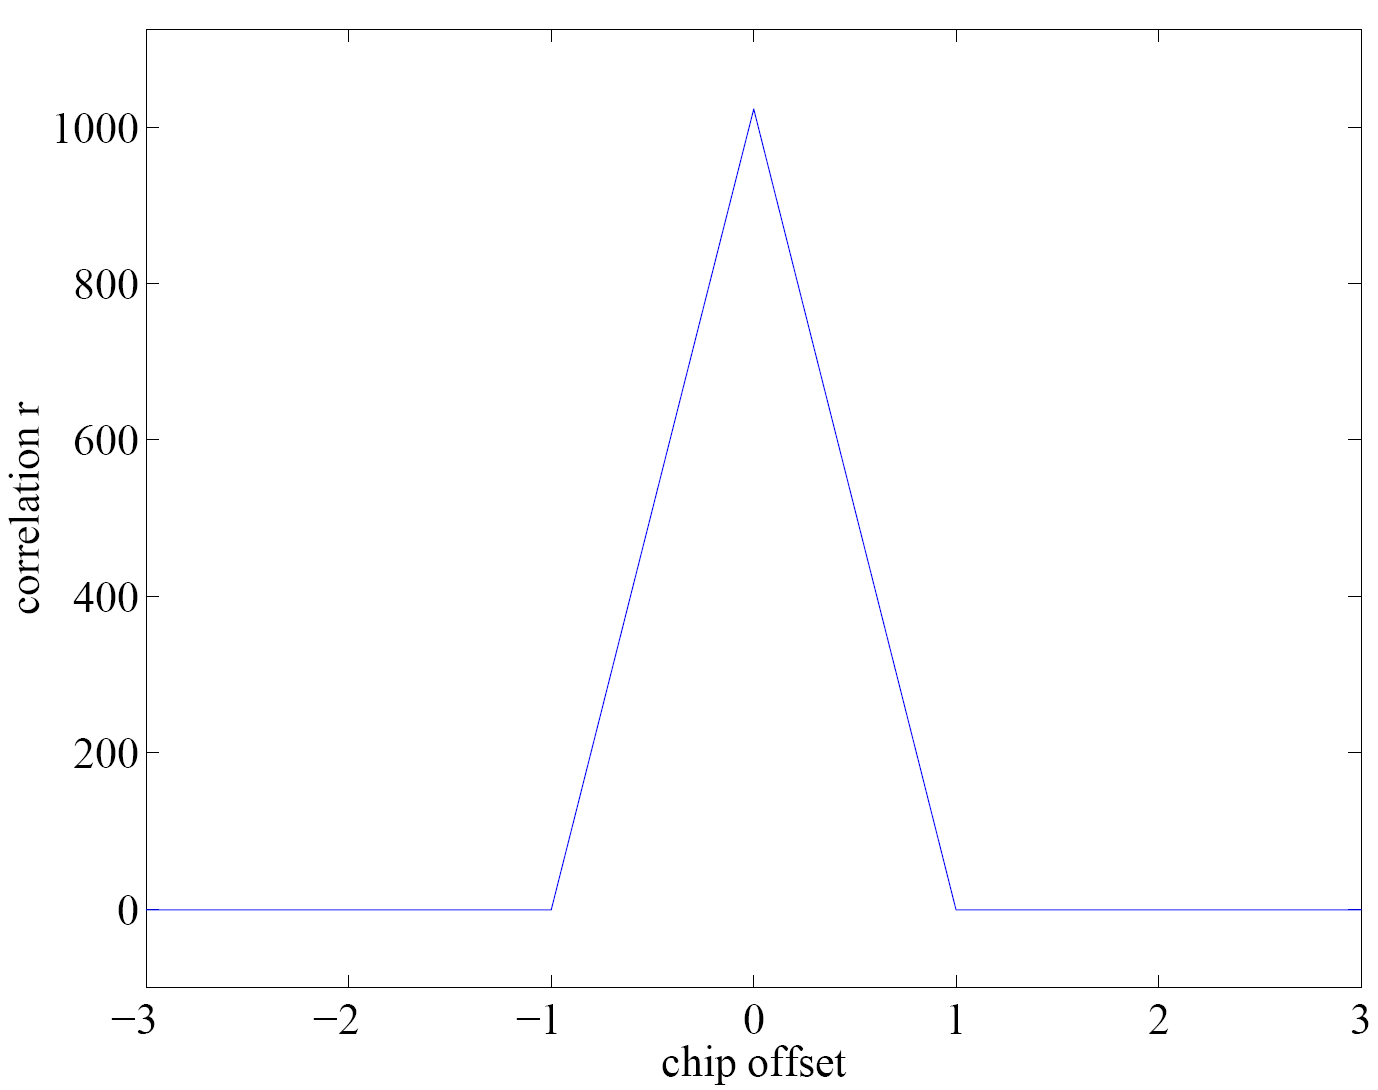
\includegraphics[width=6cm]{bilder/GPS-Autokorrelation.png}
    \end{minipage}
	\begin{minipage}{6cm}
    	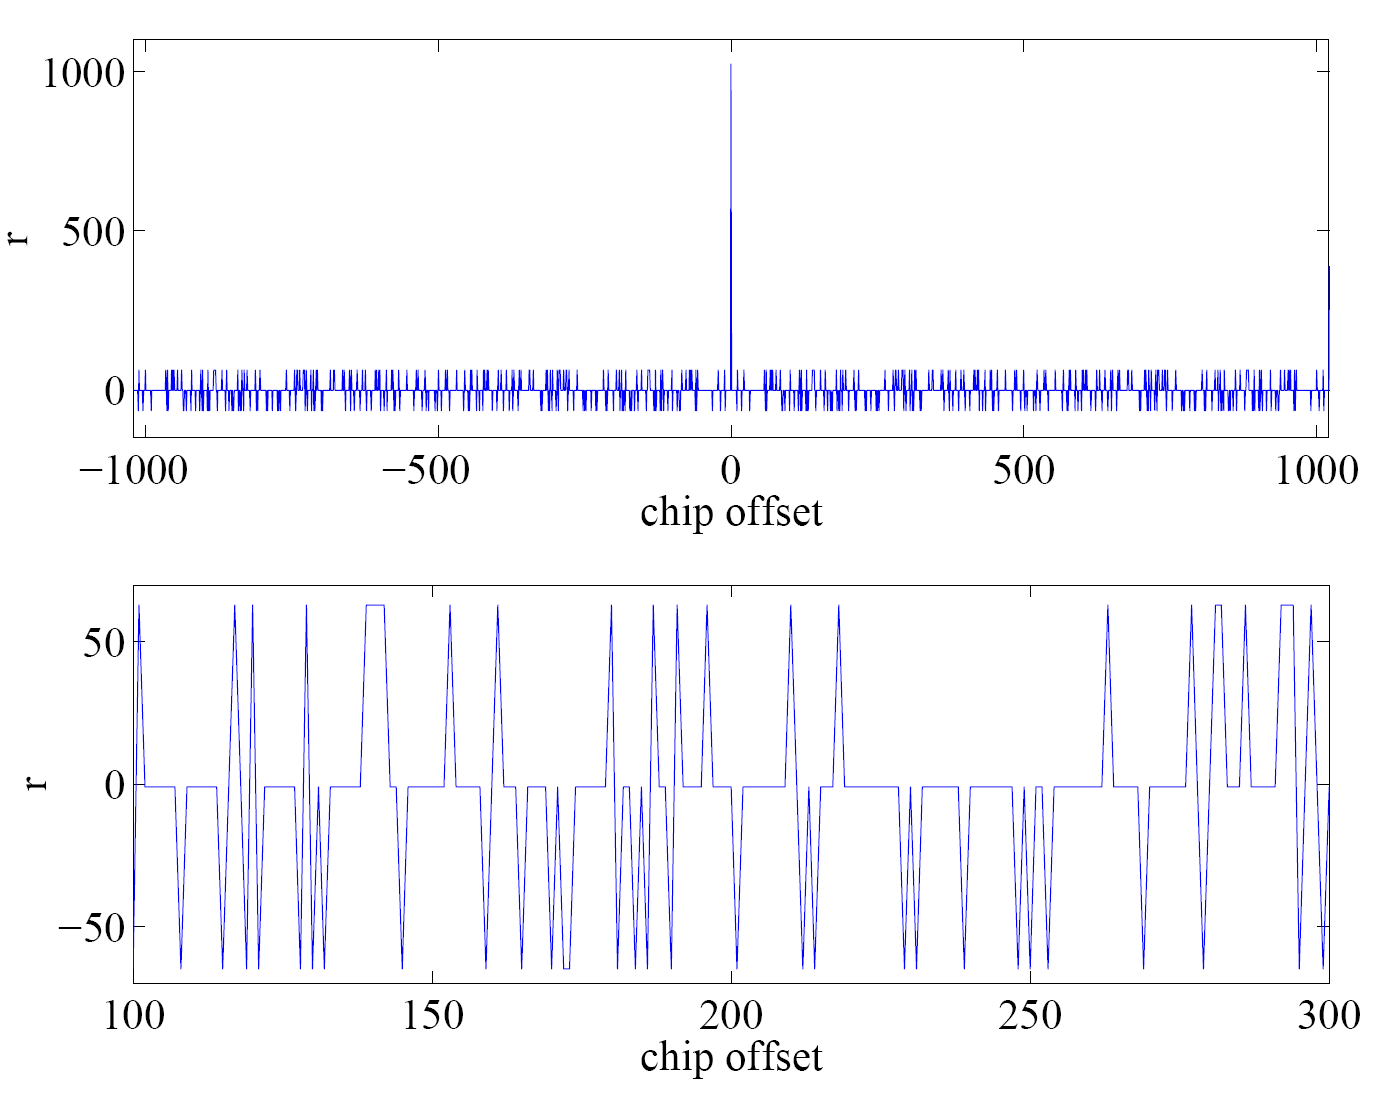
\includegraphics[width=6cm]{bilder/GPS-Autokorr_Sequenz.png}
    \end{minipage}
	\begin{minipage}{6cm}
    	Der Peak der Autokorrelation ist 1023 hoch. Da eine Sequenz immer eine
    	ungerade Anzahl an Bits hat, ist sonst der Wert bei der
    	Auto- wie auch bei der Kreuzkorrelation -1. Ausserdem k�nnen
    	auch die Werte +63 und -65 vorkommen.\\
    	Falls ein Satellitensignal um
    	$20\log_{10}(\frac{1023}{63})=23.9\text{dB}$ st�rker ist, kann eine
    	Verwechslung auftreten.
    \end{minipage}

\subsubsection{Acquisition}

	\begin{center}
    	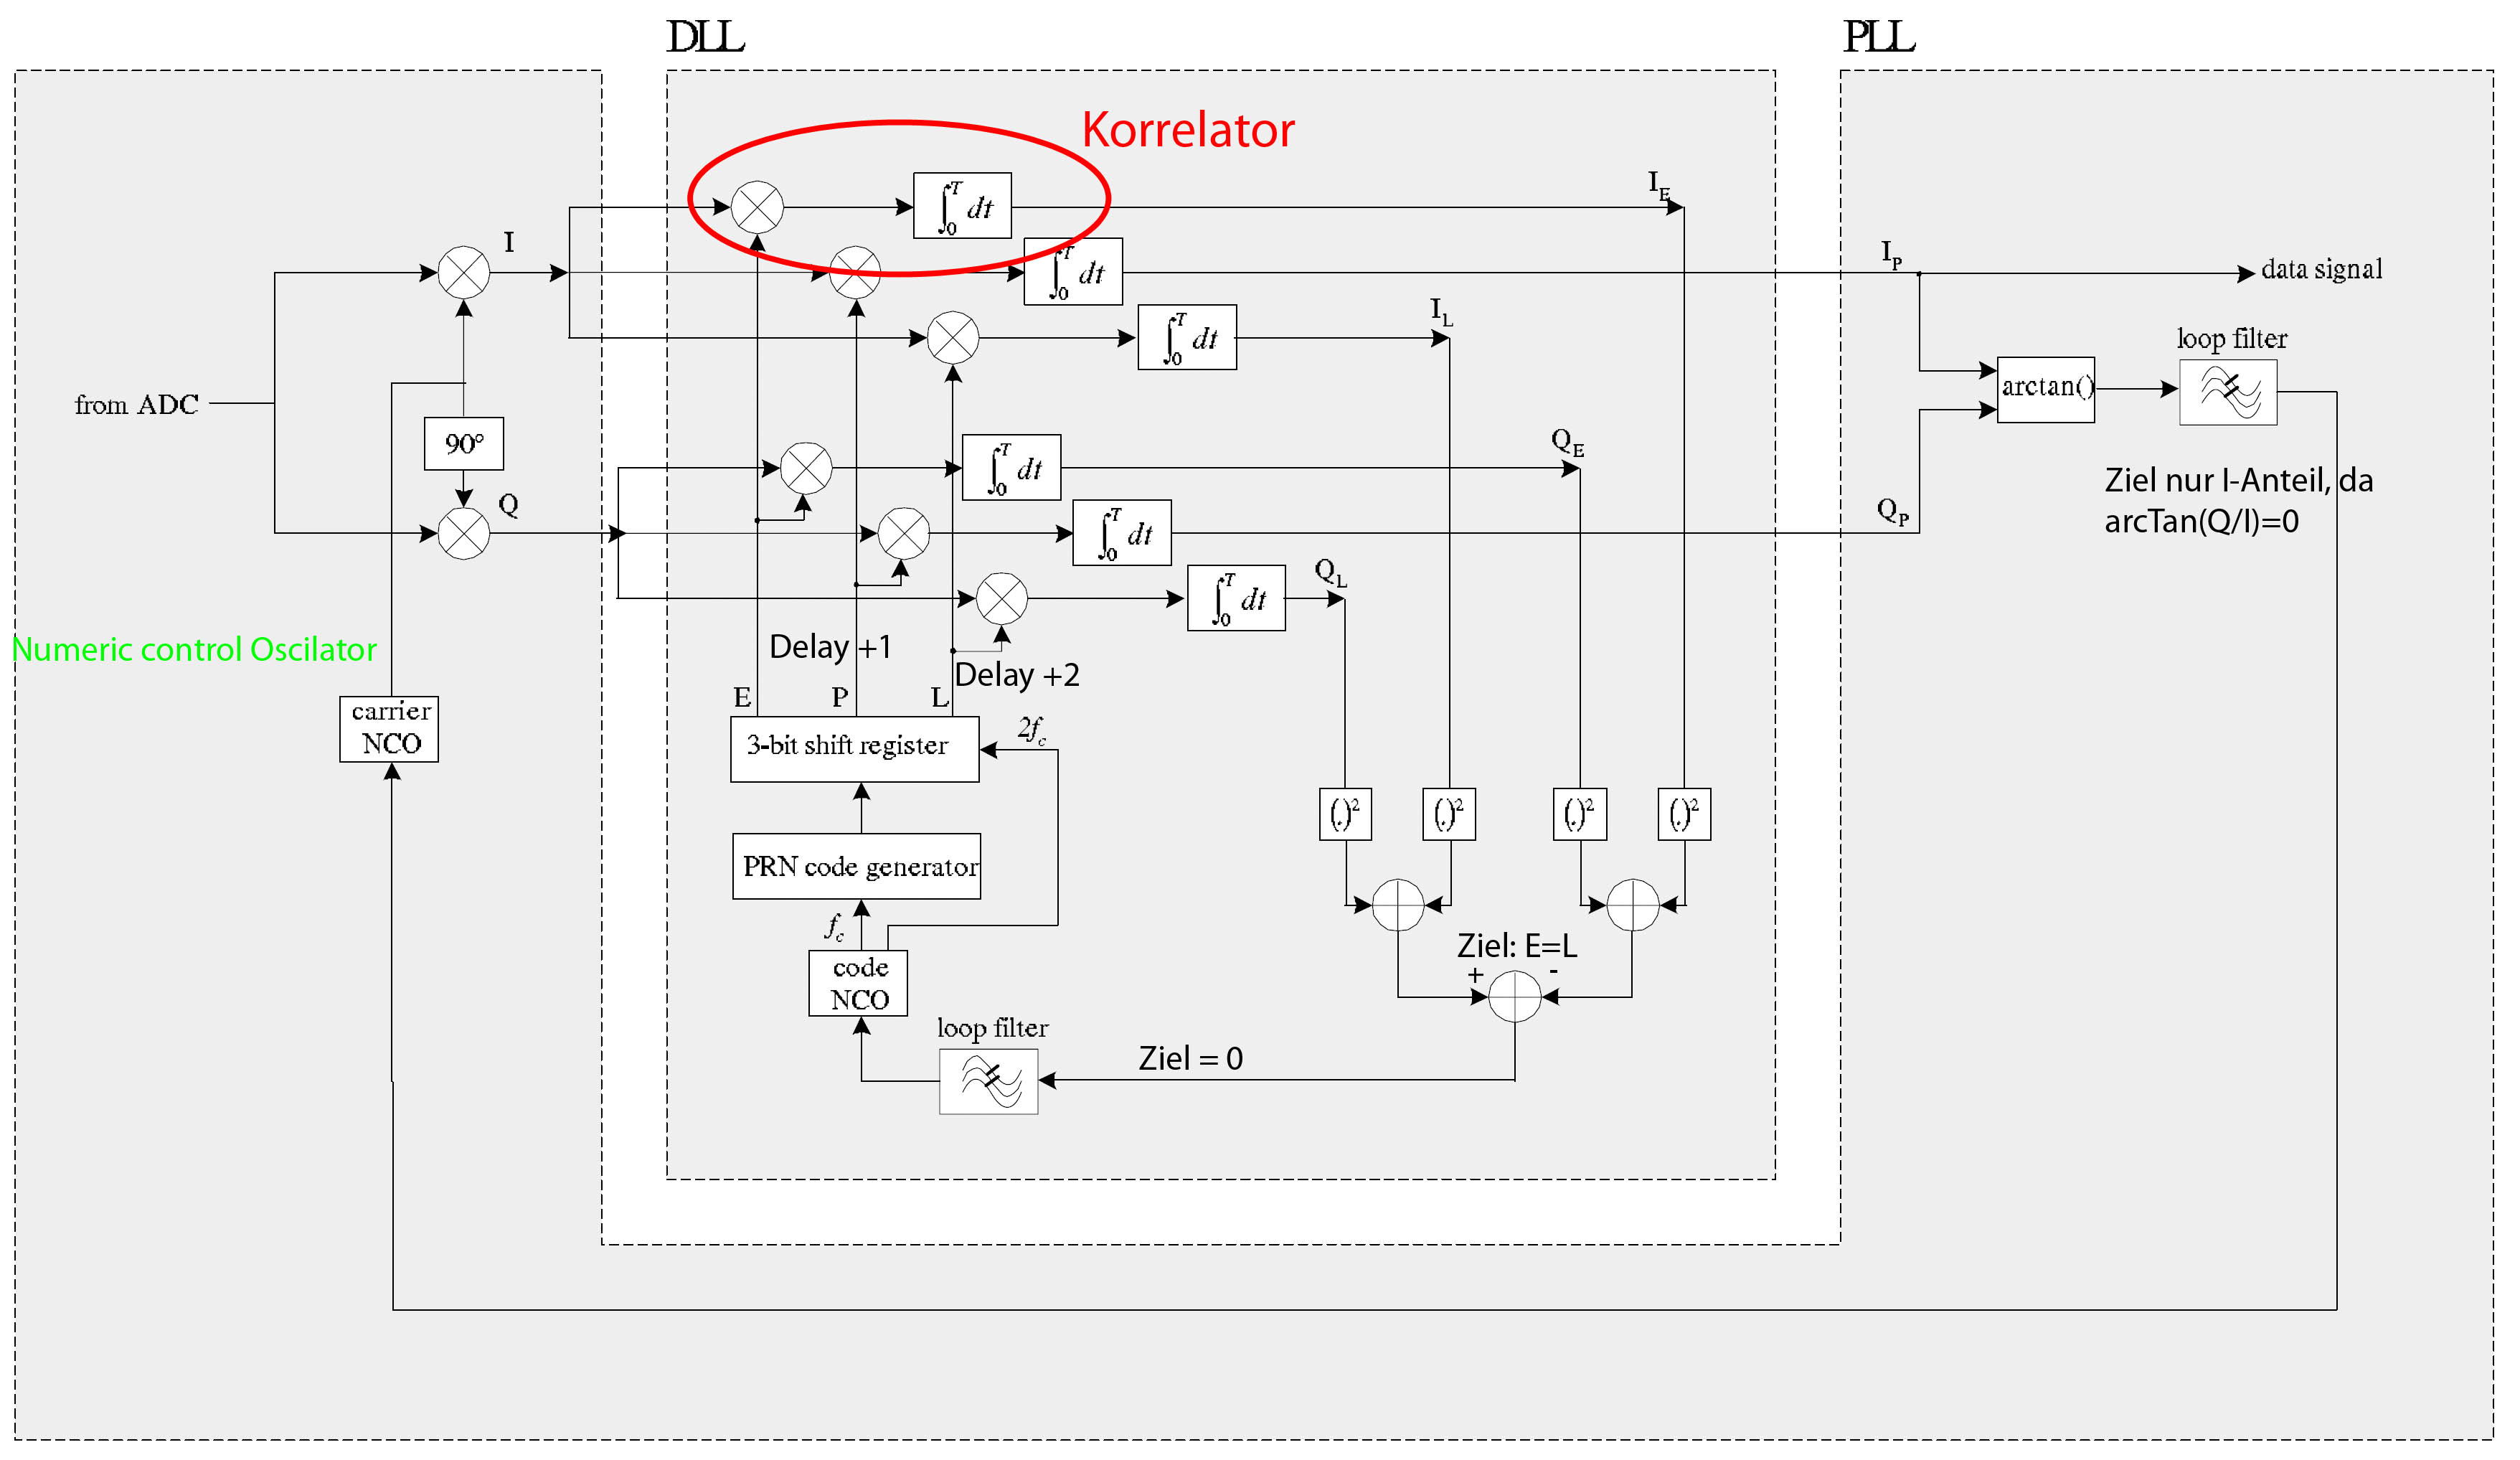
\includegraphics[width=14cm]{bilder/GPS-Phasenlock.jpg}\\
    \end{center}

	Um die Satelliten zu finden muss in 3 Dimensionen gesucht werden:
	\begin{liste}
    	\item SV nummer: 	1 bis 28 (Anz: 28)
    	\item Code Phase: 	0 bis 2045 (halbe Bitbreite) (Anz: 2046)
    	\item Frequenz:		-35kHz bis +35kHz (Da ca 20ppm = 30kHz und $\pm$ 5kHz
    	Dopplershift in je 500Hz Schritten) (Anz:141)
    \end{liste}
	Das ergibt ohne jegliches Vorwissen f�r jeden Satellit $N=2046\cdot
	141=288486$ M�glichkeiten.\\
	F�r die Auswertung muss $s=I_P^2+Q_P^2$ gerechnet werden (Korrelation) und eine
	Peakdedection vorgenommen werden.
\subsubsection{Chip resolution}
	\begin{minipage}{10cm}
	    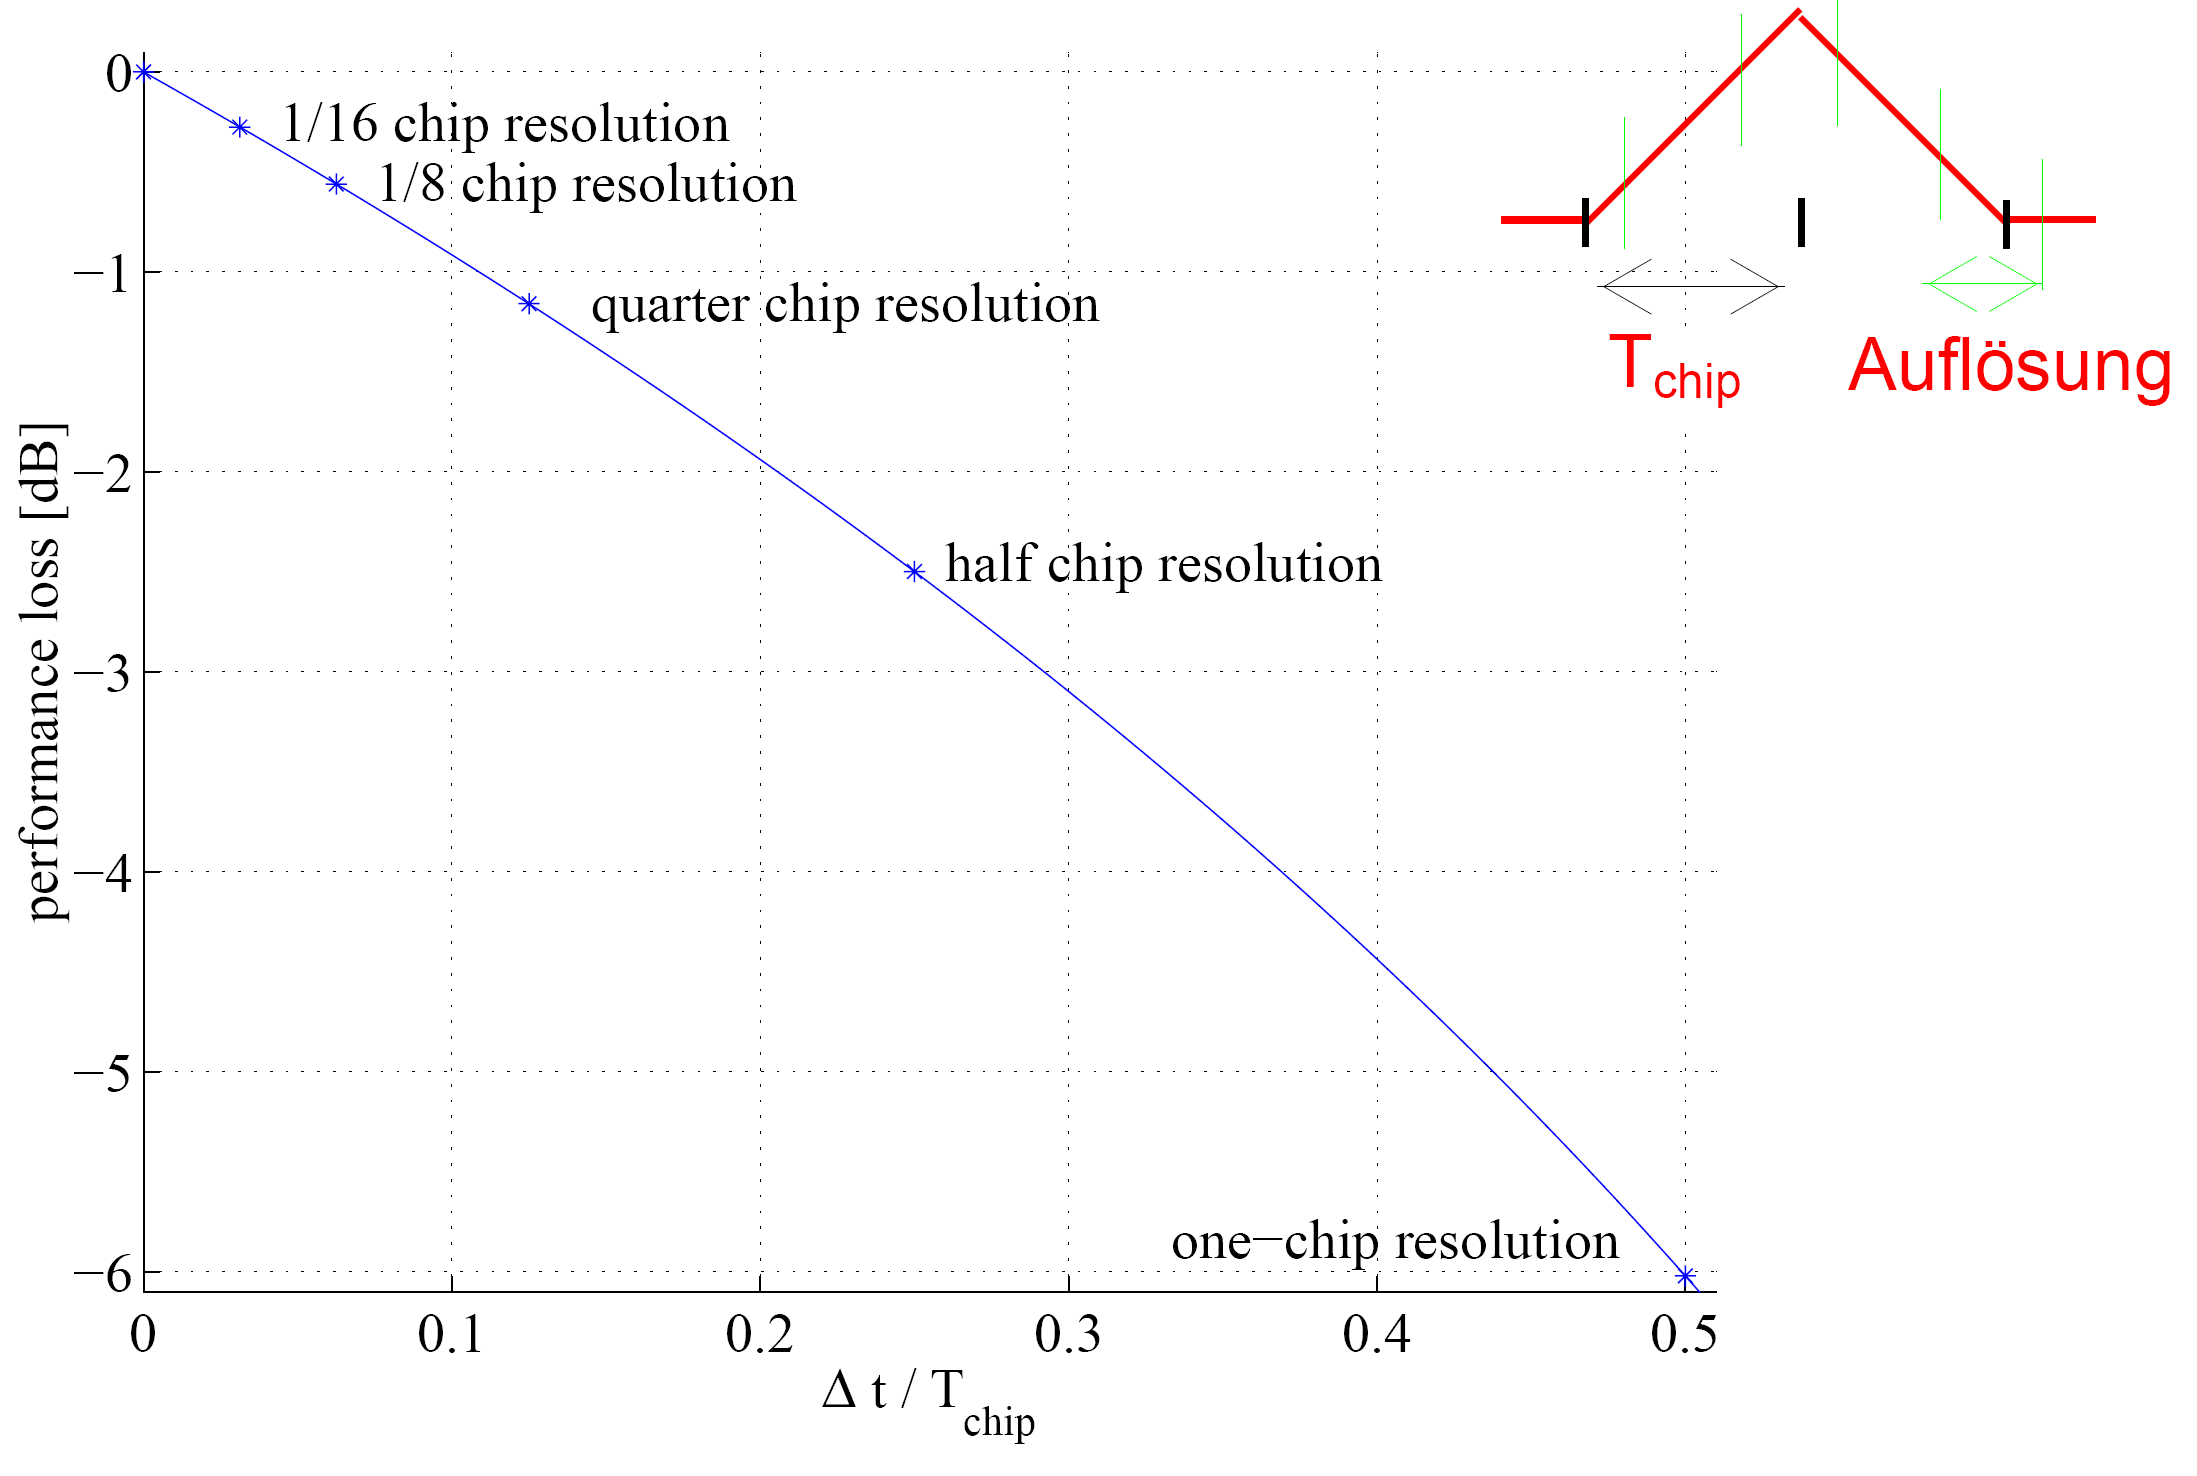
\includegraphics[width=8cm]{bilder/GPS-ChipResolution.png}
    \end{minipage}
	\begin{minipage}{8cm}
    	Da die Phase nicht genau bekannt ist, treten bei der Dedektion des
		Spitztes der Autokorrelation Verluste auf, da nicht mehr das maximum erwischt
		wird.\\
		$\text{loss [dB]}= 20 \log_{10}\left(1-\frac{|\Delta
		t|}{T_{\mathrm{chip}}}\right)$\\
    \end{minipage}
\subsubsection{Frequenz resolution}
	\begin{minipage}{8cm}
    	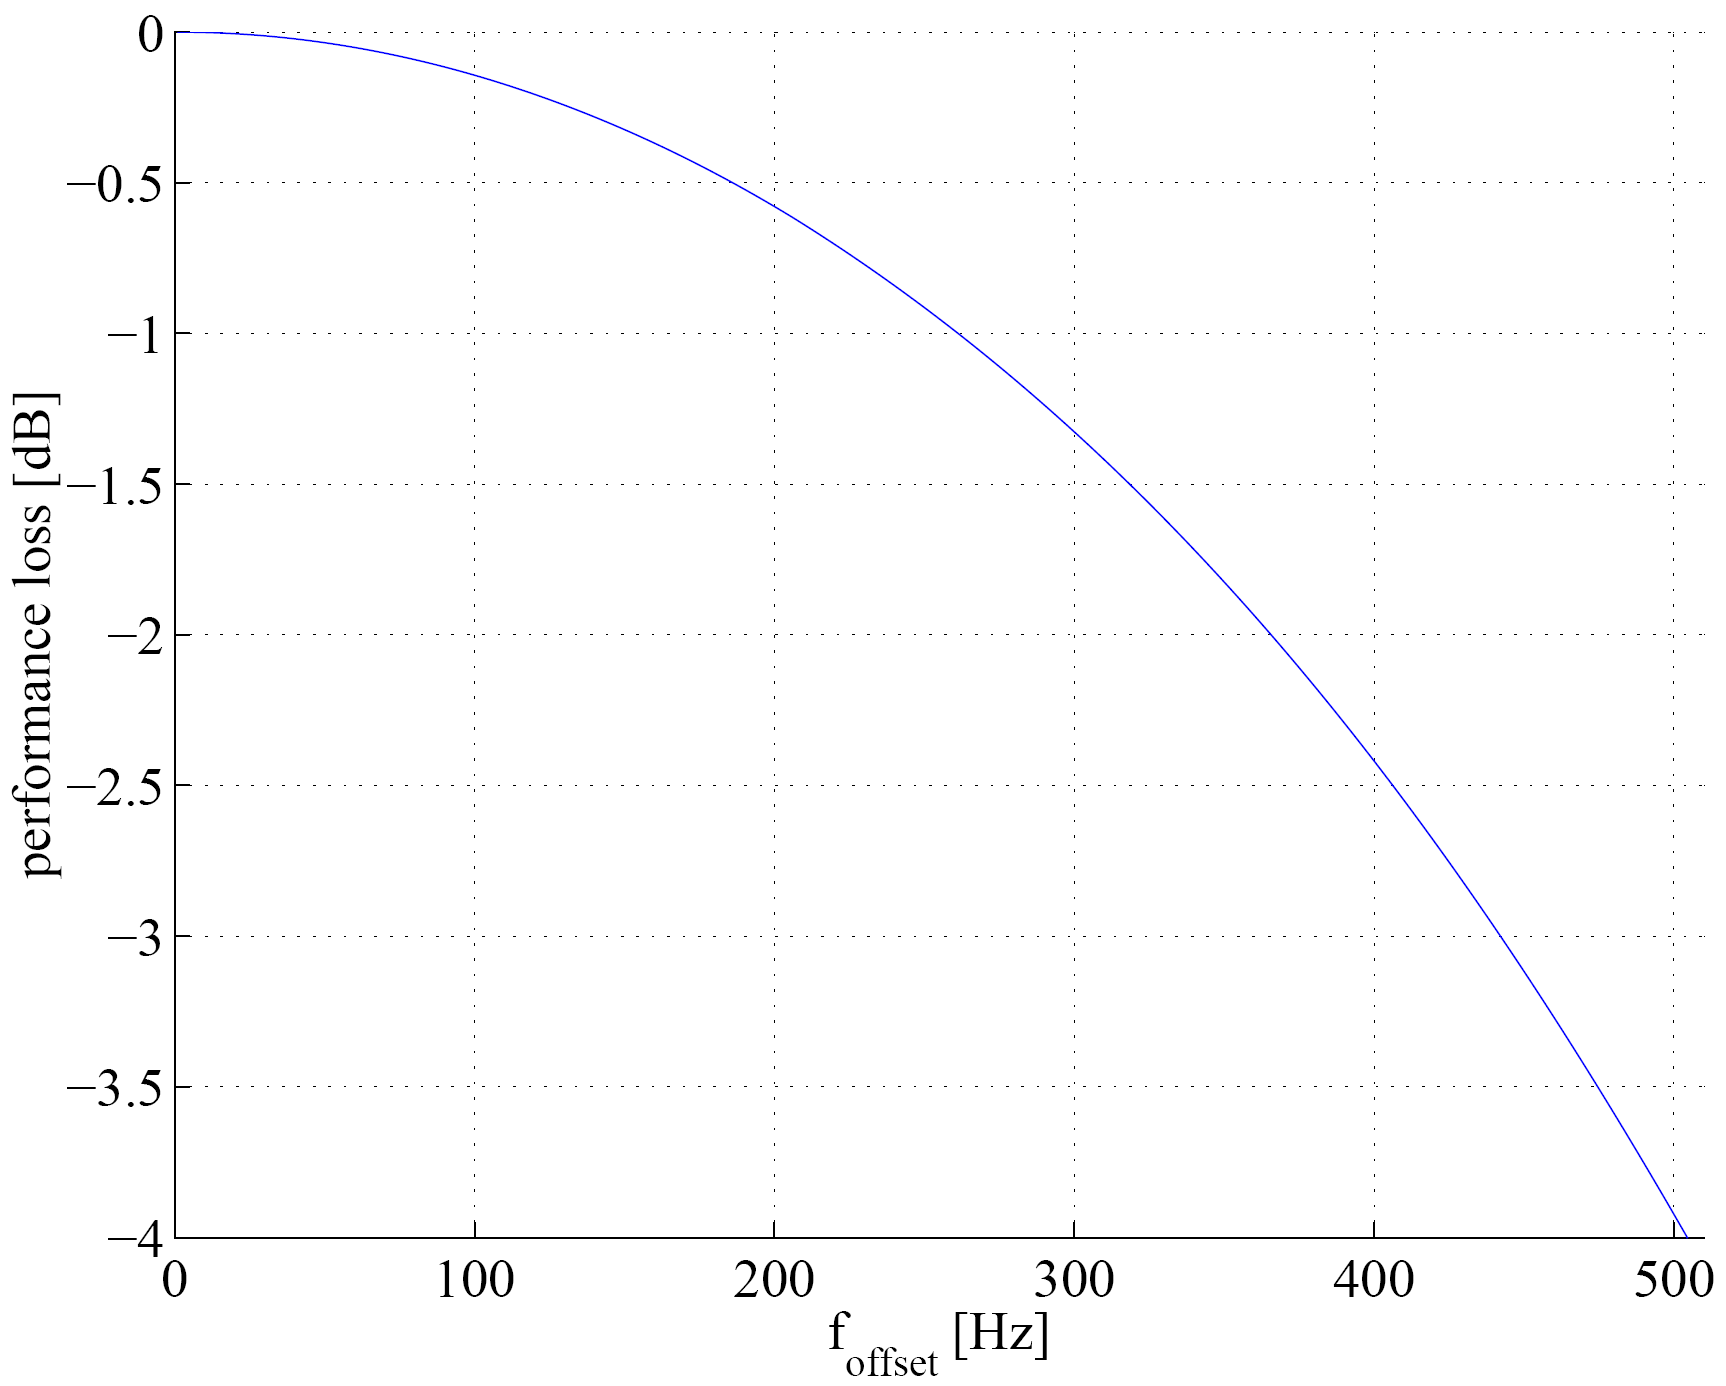
\includegraphics[width=6cm]{bilder/GPS-FrequenzResolution.png}
    \end{minipage}
	\begin{minipage}{10cm}
	    Bei einem unbekannten Doppler Shift und einer unbekannten Frequenzabweichung
		treten in der Integration Verluste auf.\\
		$\text{loss [dB]}= 20 \log_{10} \frac{\sin(\pi f_{\mathrm{offset}}T)} {\pi
		f_{\mathrm{offset}}T}$\\
     	Grafik links zeigt den Verlust nach der Integration von einer Sequenz
     	(1ms).
    \end{minipage}
    
\subsection{OFDM - Orthogonal Frequency Division Multiplexing}

\begin{tabular}{ll}
\parbox{12cm}{
Funktioniert �hnlich wie FDMA, nur werden hier zueinander orthogonal stehende
Tr�gersignale verwendet, wobei jeder Tr�ger ein Symbol (ein oder mehrere Bits)
repr�sentiert. Die Tr�gerfrequenz sind jeweils ein Vielfaches der 
$\frac{1}{T_S}=\frac{1}{Symboldauer}$. Laut Definition ist dann:
\\
$ \int^{T}_0 e^{j2\pi f_i t} e^{-j2\pi f_j t} = \int_0^{T_S} \sin (2\pi f_i
t)\sin (2\pi f_j t) dt = \left\{\begin{array}{l@{\,\,\,\,} l}
         0 , &   i\not = j, \\ 
         1 , &   i = j .   \end{array} \right.$\\
Daraus folgt, dass die bei FDMA �bliche Sicherheitsabst�nde zwischen den Tr�gern
null sind. 
       } 
&
\parbox{6cm}{
    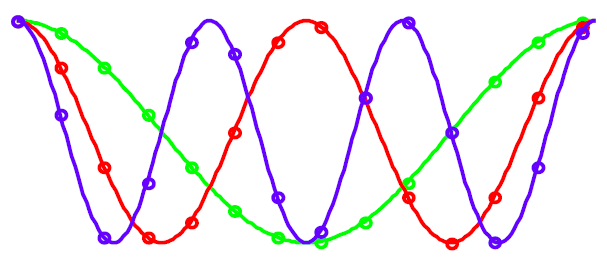
\includegraphics[width=6cm]{bilder/modulation_OFDM-orthogonal.png}\\
    \small Orthogonalit�t der Tr�ger
}       
\end{tabular}
\begin{center}
    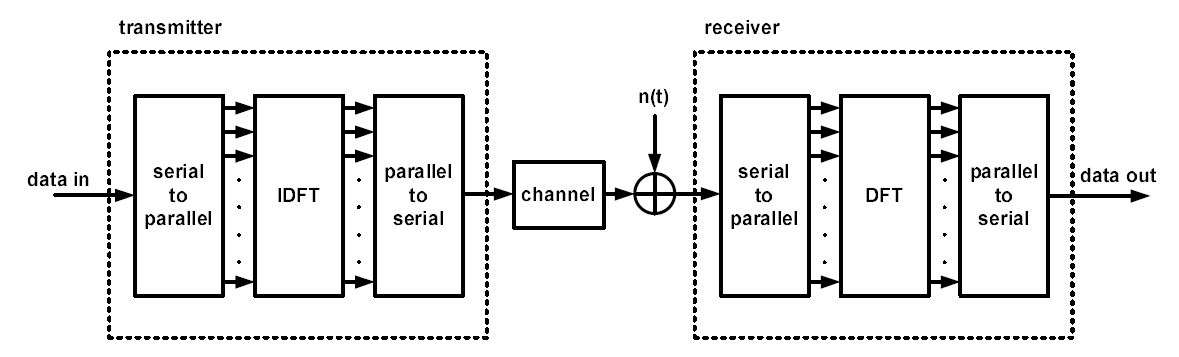
\includegraphics[width=15cm]{bilder/modulation_OFDM-schematic.png}\\
    \small Blockschaltbild - OFDM Sender und Empf�nger
\end{center}

\begin{tabular}{lll}
\parbox{4cm}{
$$\frac W{B_{\text{coh}}} \ll N_c \ll WT_{\text{coh}} $$ 
$$ T_{\text{coh}} < \dfrac{N_c}{R} = T_{\text{Subcarrier}} $$
       } 
&
\parbox{5cm}{
   $W$: Gesamtbandbreite \\
   $\dfrac{W}{N_C}$: Subcarrier Bandbreite \\
   $R$: Symbolrate (gesamtes Band)
}       
&
\parbox{9cm}{
   $N_C$: Anzahl Subcarrier bzw. Kan�le \\
   $B_{\text{coh}}$: Koh�renzbandbreite \\
   $T_{\text{coh}}$: Koh�renzzeit (Zeitinvarianz �bertragungskanal)
}       
\end{tabular}

Im Vergleich zur seriellen �bertragung ergibt sich bei der gleichen
�bertragungsrat eine viel l�ngere
Symbolzeit, da die Daten parallel �bertragen werden ergibt. Dies
erm�glicht es den Subcarrier gegen�ber Eintr�gerverfahren, viel weniger
Bandbreite zu nutzen. So wird die Symboldauer viel l�nger, so dass die Kanal
- Laufzeit bzw. Echos einen viel kleiner Einfluss hat.
\\
\subsubsection{Nachteil}
\textbf{PAPR}:\\
Der PAPR - Peak-to-Average-Power Ratio ist ist teils sehr gross.
PAPR =  Verh�ltniss von Spitzen in der Ausgangsleistung zu Durchschnittleistung.
$PAPR = \frac{P_{Peak}}{P_{Av} } $ f�r OFDM ohne Korrektur mit BPSK:
$PAPR=\frac{N^2 P_{sub}}{N P_{sub}}=N$\\ \\
M�glichkeiten den PAPR zu verkleinern:
\begin{liste}
	\item 	\textbf{redundant selection:} ein Symbol kann 2 unterschiedliche QAM
	Positionenen einnehmen. (je nachdem hat das Symbol eine Phasen, welche dann ein besseres
	PAPR ergibt)
	\item 	\textbf{coding technics:} Schon im digitalen Bereich werden
	Konstellationen mit grossen Peaks vermieden.
	\item	\textbf{soft clipping beim power amplifier:} Die Spitzen werden langsam
	unterdr�ckt (es gibt Oberschwingungen welche dann wiederum Fehler ergeben). Mit
	einer Fehlerkorrektur k�nnen diese jedoch wieder herausgerechnet werden.
	\item	\textbf{tone/frequnz reservation:} falls bei den Datenfrequenzen alle
	+, die Reservent�ne werden - gesetzt\\
\end{liste}

Problem der \textbf{Multidimensional Interference (MDI)}:
\begin{liste}
    \item \textbf{Intersymbolic Interference (ISI)} \\
            Symbole �berlappen sich im Zeitbereich (wegen Faltung mit Impulsantwort des Kanals - Laufzeit, Echo, usw.)
    \item \textbf{Inter Channel Interference (ICI)} \\
            Subcarrier sind nicht mehr orthogonal. Ursachen ist unter
            anderem, dass der Kanal nicht Zeitinvariant ist. $\Rightarrow$ Es
            gibt Frequenzverschiebungen.
            Einen weiteren Ursache kommt vom ISI:\\
\end{liste}

\begin{tabular}{lll}
	\parbox{6cm}{ 
    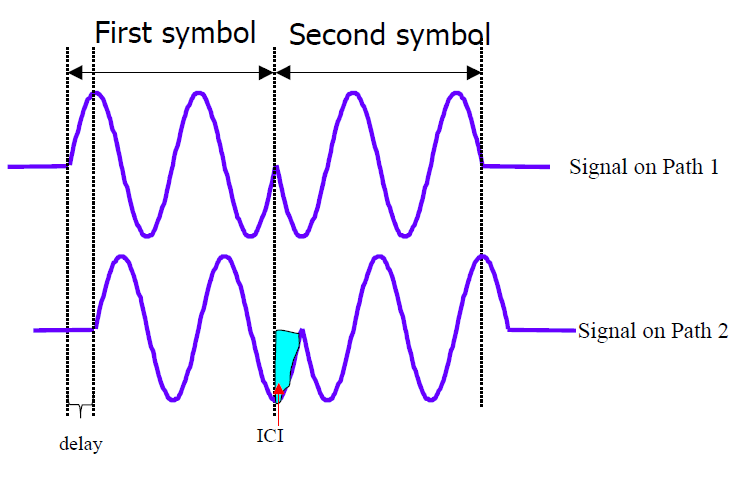
\includegraphics[width=6cm]{bilder/modulation_OFDM-ICI.png}\\
	}    
	& \parbox{6cm}{Ein nicht-sinusf�rmiges Signal (Bild links) h�tte mehrere/h�here
	Frequenzkomponenten zur Folge, welche in andere Subcarrier �berlappen w�rden -
	\textbf{ICI}. Um dies zu verhindern wird das Signal mit einem sogenannten \textbf{Cyclic
	Prefix} (Bild rechts) versehen, sodass ein reines sinusf�rmiges Signal
	resultiert. \\	
	} &
	\parbox{6cm}{
	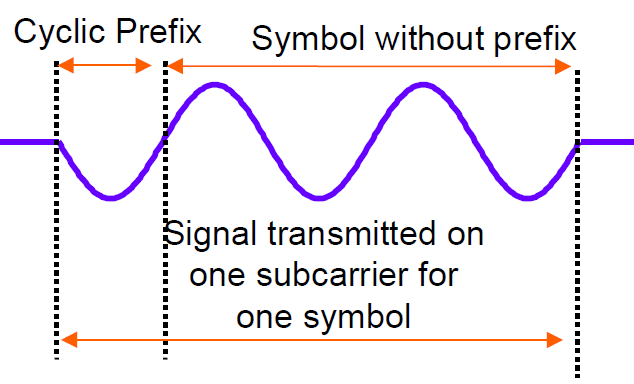
\includegraphics[width=6cm]{bilder/modulation_OFDM-prefix.png}\\ }       
\end{tabular}



\section{Modulation}
Die analogen continuierlichen Modulationsarten wie AM, FM und PM werden hier
nicht behandelt. Es wird von digitalen Daten ausgegangen.

\subsection{Komplexes Basisband }
Generell ist ein RF- Signal symmetrisch bez�glich des Nullpunktes
($A_1=A_{-1}$)nicht jedoch bez�glich des RF Tr�gers. Dies hat zur Folge, dass
das demodulierte Signal nicht mehr symetrisch zu Null ist, was bedeutet, dass
es ein komplexes Spektrum ist. $s_{RF}(t)=\Re(s_{bb}(t)e^{j2\pi f_{RF}t})$\\
\begin{tabular}{lll}
	\parbox{5cm}{
		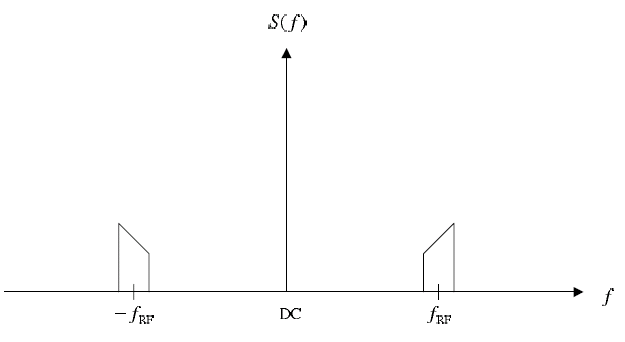
\includegraphics[width=5cm]{bilder/modulation_RFSpektrum.png}
	}
	&$\Longrightarrow$
	&\parbox{5cm}{
		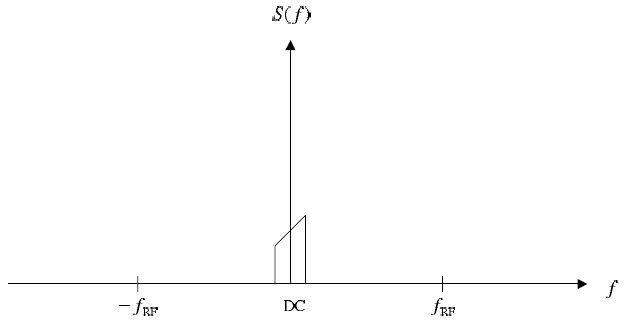
\includegraphics[width=5cm]{bilder/modulation_BBSpektrum.png}
	}
\end{tabular}

\subsection{BPSK - Binary Phase Shift Keying  }
\begin{tabular}{ll}
	\parbox{10cm}{
		\begin{tabular}{ll}
			BPSK&= 2-PAM \\
			Phase $\in \{-180^o, 0$\} &= Amplitude $\in \{-1, 1\}$
		\end{tabular}\\
		Bild rechts zeigt Amplitude und Phase des Basisbandes genau zur sampling
		time.\\
	}
	&
	\parbox{5cm}{
		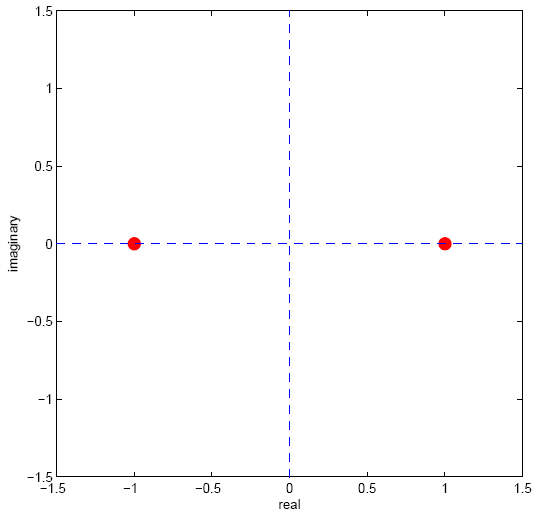
\includegraphics[width=5cm]{bilder/modulation_constellationBPSK.png}
	}
\end{tabular}
\subsection{M-PAM - Pulse Amplitude Modulation }
M kommt von M- Zust�nden, welche die Amplitude annehmen kann. Dadurch k�nnen
$N=\log_2(M) [\frac{bits}{Symbol}]$ �bertragen werden. Durch die Abstufung wird
die Effizienz gesteigert. Da PAM ein reelles Spektrum besitzt ist auch das
RF-Signal symmetrisch zum Tr�ger, was jedoch die Bandbreiteneffizient stark
vermindert. M�gliche Verbesserungen:\\
\begin{liste}
	\item Zus�tzlicher Imagin�ranteil $\Longrightarrow$ QAM
	\item Gr�sseres M (Nachteil: gr�ssere Fehlerwahrscheindlichkeit und
	immernoch symetrisch)
	\item Eliminierung des einen Frequenzbandes(z.B mit SSB)
\end{liste}

\subsection{M-QAM - Quadratur Amplitude Modluation }
\begin{tabular}{ll}
\parbox{10cm}{
	Bei QAM wird die Phase und Amplidue ver�ndert. Um eine optimale Ausn�tzung zu
	erhalten soll $M=2^n$ gew�hlt werden, wobei $n \epsilon \mathbb{N}$ und 
	$n=N=\frac{bit}{Symbol}$ist.\\
	Falls n gerade dann ergibt es ein vollst�ndiges Viereck.\\
	Bei n ungerade ergibt sich ein Viereck ohne die Ecken.\\
	Spezialfall: 4- QAM = QPSK\\
	Das Problem f�r die MobKom an QAM ist, dass sich die Amplituded�mpfung sehr
	stark und relativ schnell �ndern kann. Deshalb kann man keine Information als
	Amplituden�nderung senden, was dann nur noch eine Phasenverschiebung (M-PSK)
	zur Folge hat.} 
	& \parbox{8cm}{
	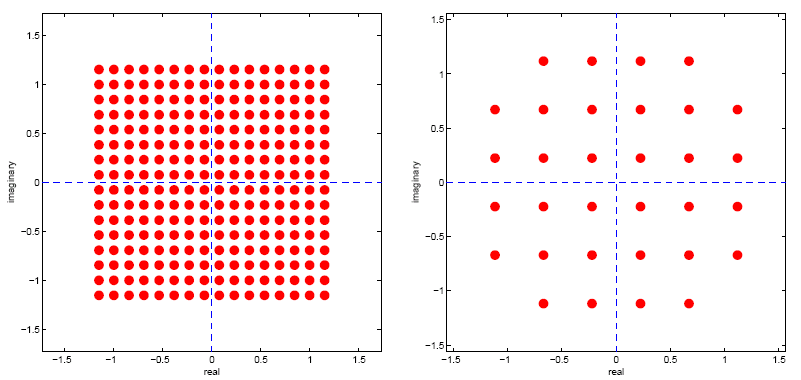
\includegraphics[width=8cm]{bilder/modulation_constellationQAM.png}\\ 256-QAM und 32-QAM
}
\end{tabular}

\subsection{M-PSK - Phase Shift Keying }
\begin{tabular}{ll}
\parbox{10cm}{
Spezielle Formen:\\
\begin{liste}
 \item Bei \textit{D}PSK kommt es nicht mehr auf die
	absolute Phase an, sondern nur noch auf den Phasensprung von Symbol zu Symbol
	(z.B. je $\frac{\pi}{4}$). So ist keine Referenz zur Nullphase n�tig.
 \item \textit{$\frac{3\pi}{8}$} oder \textit{EDGE-Modulationschema} wird bei
 GSM eingesetzt. Der Vorsatz \textit{$\frac{3\pi}{8}$} bedeutet, dass zu
 einem normalen Phasensprung (hier $n \frac{\pi}{4}$ nochmals einen Offset
 von $\frac{\pi}{8}$ hinzu kommt. Dies hat zur Folge, dass die komplexe
 Amplitude nie null wird. (siehe Bild)
\end{liste}


}
&\parbox{6cm}{
    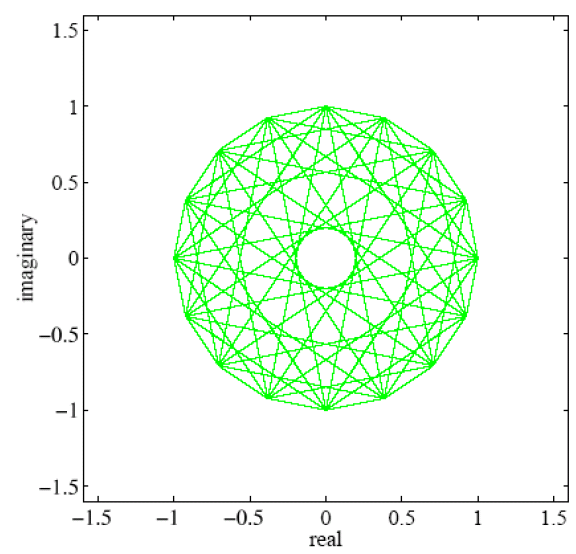
\includegraphics[width=6cm]{bilder/modulation_constellationEDGE.png}\\
    $\frac{3 \pi}{8}$ 8-PSK

}
\end{tabular}

\subsection{Gray- Code }
\begin{tabular}{ll}
	\parbox{8cm}{
		Der Vorteil des Gray Codes gegen�ber der normalen bin�ren Codierung ist, dass
		bei einem Fehler nur ein Bit falsch wird und nicht gerade alle, wie das Bild
		rechts zeigt.\\
        Bsp. aus Pr�fung (12. M�rz 2007): Vergr�sserung des BER, wenn bei QPSK
        die bin�re Standardcodierung statt der Gray-Codierung verwendet wird.
        
        Gray: BER = SER/2 \\
        Bin�r: BER = SER/2 + SER/4 \\
        Verschlechterung: $\Rightarrow 3/2$   \\ \\
        
        F�r Gray-Code gilt: $\text{BER} \approx
        \dfrac{\text{SER}}{n_{\text{bits}}}$ } &\parbox{10cm}{
		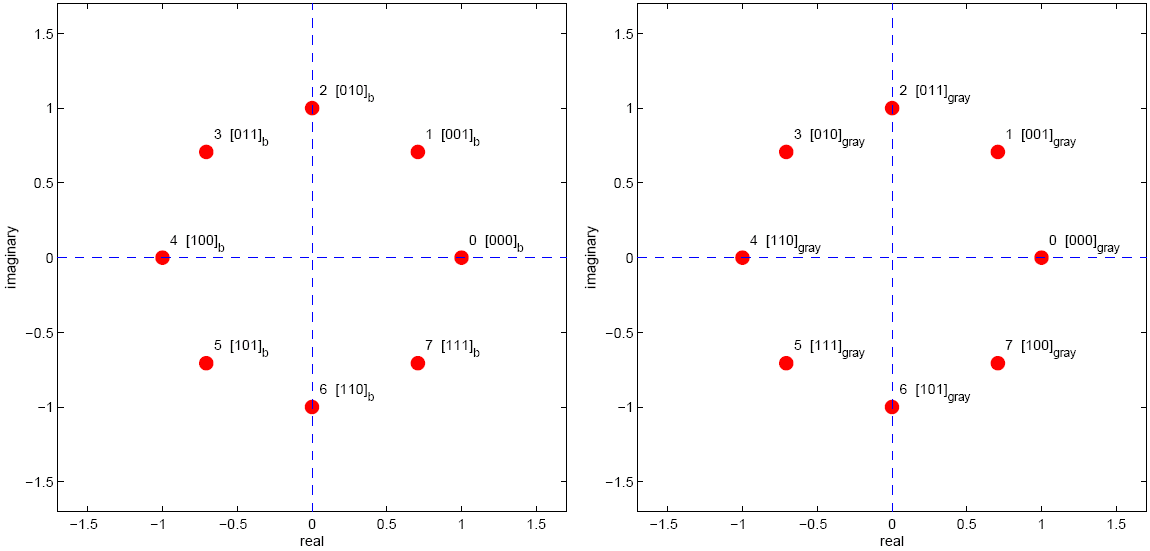
\includegraphics[width=10cm]{bilder/modulation_PSKmitGray.png}\\
		8-PSK ohne bzw. mit Gray- Code
	}
\end{tabular}

\begin{tabular}{ll}
	\parbox{9cm}{
		\subsection{FSK - Frequency Shift Keying }
		Bei FSK wird ein bin�res Signal frequenz-moduliert. Das heisst,
		es switscht (hihi) zwischen zwei Frequenzen, dies wird meist mit Hilfe eines
		VCO gemacht.\\
		Kenngr�sse ist der Modulations Index: \\
		$h=\dfrac{\Delta f}{f_{\text{data}}}=\dfrac{f_{\text{max}} -
		f_{\text{min}}}{f_{\text{data}}} =\dfrac{n_{\text{T-max}} -
		n_{\text{T-min}}}{n_\text{T}}$ \\ Bei einem \textbf{h von 0.5 }spricht man von
		\textbf{Minimum Shift Keying (MSK)} oder \textbf{Fast} Frequency Shift Keying
		\textbf{(FFSK)}. Tr�gerfrequenzen k�nnen orthogonal sein, solange der
		Modulationsindex das Minimum $h_{\text{min}}$ nicht unterschreitet. \\ $h_{\text{min}} =
		\begin{cases} 1   & \text{unkoh�rente Detektion} \\                                
                                0.5   & \text{koh�rente - phase
                                synchron - Detektion} \end{cases}$\\
        F�r unkoh�rente Detektion sind die beiden Tr�ger orthogonal, wenn gilt:
        \\
        $    \Delta f = \frac{1}{T_{\text{data}}} \cdot n , \qquad n \in \lbrace
        1, 2, 3, \ldots \rbrace $
	}
	&\parbox{9cm}{
	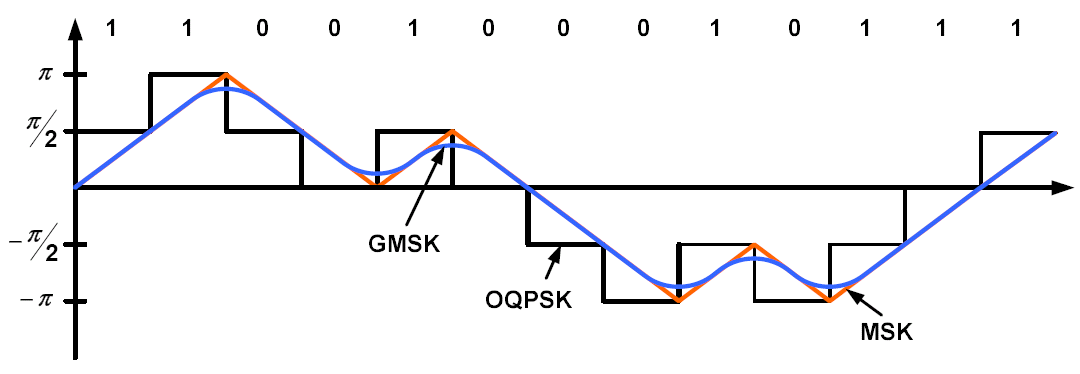
\includegraphics[width=9cm]{bilder/modulation_phasenverschiebungGMSK_MSK.png}\\
	Phasenverschiebung des MSK bzw GMSK. }
\end{tabular}
     
        
\subsection{GMSK - Gaussian Minimum Shift Keying }
Das GMSK ist ein MSK mit einem gauss'schen premodularen Filter. Es besitzt eine
konstante Amplitude und eine grosse spektrale Effizient.
        

\subsection{OQPSK - Offset Quadratur Phase Shift Keying \formelbuch{75, 68}}
Das OQPSK ist eine Sonderform der Quadraturphasenmodulation
	

\subsection{TCM - Trellis Coded Modulation}
\subsubsection{Covolutional Coding - Faltungs Code}
Ein Faltungs Code besitzt zur Logikschaltung zus�tzlich noch Memory, so dass
nicht nur der aktuelle Eingang sondern auch noch n- Vorherige Eing�nge zum
Ausgang verrechnet werden. Es gibt m unterschiedliche Ausg�nge. 
Je nach Vorgeschichte, k�nnen nur noch ganz bestimmte Kombinationen auftreten,
was dann die Decodierung besser macht.\\
\begin{minipage}{9cm}
	Beispiel mit k=1; n=2; m=2 => 1/2 codierung\\
	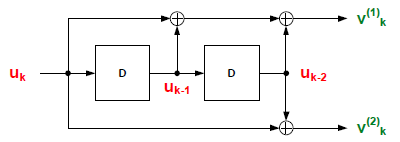
\includegraphics[width=9cm]{./bilder/covolutionSchemata.png}
\end{minipage}
\hspace{5mm}
\begin{minipage}{8cm}
\vspace{4mm}
	mit dazugeh�rigem Encoder State Diagram\\
\hspace{5mm}
	\includegraphics[width=6cm]{./bilder/covolutionStateDiagram.png}
\end{minipage}

\subsubsection{Decodierung}
Eine gute Variante die FaltungsCodes zu dekodieren ist dies mit einem Trellis
Diagram zu machen: \\
\begin{minipage}{10cm}
	\begin{liste}
		\item Zuerst Punkte entsprechend der m�glichen Speicherinhalten einzeichnen.
		\item M�gliche Verbindungen einzeichnen.
		\item Soll Werte einzeichnen (z.B. 0/00).
		\item Fehler zu den einzelnen Punkten eintragen (ev. die Euklidische Distanz).
		\item Wenn zwei Wege zu einem Punkt kommen, den h�herwertigen Weg streichen.
		\item Am Schluss den Weg nehmen der den kleinsten Fehler ergibt.
	\end{liste}
\end{minipage}
\begin{minipage}{9cm}
	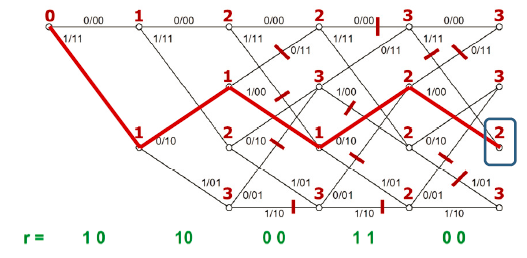
\includegraphics[width=9cm]{./bilder/Trelli.png}
\end{minipage}

\subsubsection{Euklidische Distanz}
\begin{minipage}{13cm}
	Die \textbf{euklidische Distanz} ist der Abstand zwischen zwei
	unterschiedlichen Modulationspositionen.\\
	Die \textbf{freie euklidische Distanz} ist der minimaler Abstand zwishcen zwei
	unterschiedlichen Modulationspositionen in der ganzen Modulation.\\
	$d^2_{free}=\min \limits_{a_k \neq a_{k}^{'}} \sum \limits_k
	d^2(a_k,a_{k}^{'})$\\
	zB.	$d^2_{min}=1 + 1 -2\cos (\alpha)= 2-\sqrt{2} = 0.586$\\
	Der \textbf{Coding Gain} ist um welchen Faktor der SNR schlechter sein darf.\\
	$G = \frac{d^2_{free,coded}}{d^2_{min, uncoded}}$
\end{minipage}
\begin{minipage}{6cm}
	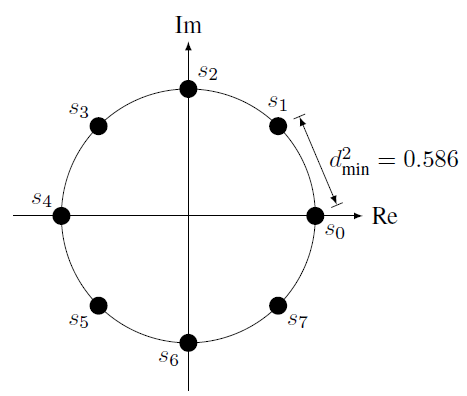
\includegraphics[width=6cm]{./bilder/EuklidischeDistanz.png}

\end{minipage}
\subsubsection{TCM}
Ziel ist es die Modulation und die Fehlercodierung als Einheit zu betrachten.
Beim TCM wird der Faltungs Code und PSK bzw QAM miteinander kombiniert. So wird
je nach dem nicht mehr eine Codekombination nicht mehr m�glich sondern eine
bestimmte Modulationsposition.\\
\begin{minipage}{9cm}
	zB. Einem QPSK wird auf ein 8PSK mit einem 2/3 Trelli erweitert. Dadurch
	entstehen einzelne Partitionen, in welcher die Modulation sein kann:\\
	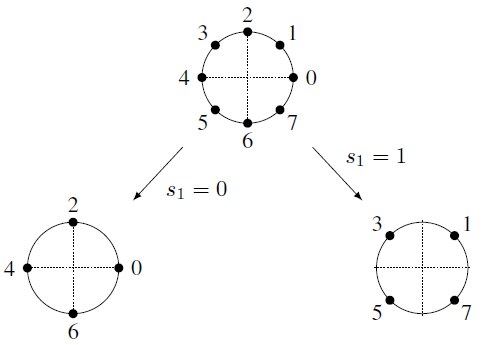
\includegraphics[width=9cm]{./bilder/Partition8PSK.png}
\end{minipage}
\begin{minipage}{9cm}
	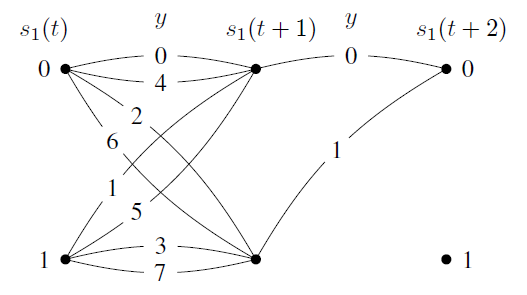
\includegraphics[width=9cm]{./bilder/Trelli2_3.png}\\
	Die Euklidische Distanz nimmt nun zu. zB. \\
	Der Abstand zu 0;0 ist im minimum 2;1 \\
	$d^2_{free}=d^2(0,2) + d^2(0,1) = 2 +	(2-\sqrt{2})=2.5858$\\
	Da die Euklidishce Distanz bei QPSK nur 2 ist ist der Coding Gain:
	$G=\frac{2.5858}2$

\end{minipage}


	
\subsection{Modulationskriterien}
Es gibt 3 Wege um die Fehlerwahrscheinlichkeit
herauszufinden:
\begin{liste}
	\item Austesten und messen (dauert bei kleiner Fehlerwahrscheinlichkeit so
	lange, bis ein vern�nftiges Resultat erreicht wird).
	\item Simulieren (dazu ist ein gutes Model n�tig, kann unter Umst�nden gleich
	lange dauern wie austesten).
	\item Analystisch mit Symbol- und Biterrorrate.
\end{liste}
\subsubsection{SER - Symbolfehlerrate }
\begin{tabular}{ll}
\parbox{8cm}{
    \includegraphics[width=8cm]{bilder/modulation_AWGN.jpg}
    }
& \parbox{9cm}{
	Die Symbolfehlerrate wird unter anderem verursacht durch das thermische
	Rauschen (AWGN). Dieses hat die Energie\\ 
	$\sigma^2=\frac{N_0}{2}$ \\
	\\
	Die Fehlerwahrscheinlichkeit ist $P_E=Q(\sqrt{\frac{2 E_S}{N_0}})$ mit $a_1 =
	E_S, a_2 = -E_S$ und $\lambda_0 = 0$\\
    }
\end{tabular}

\small
\renewcommand{\arraystretch}{0.6}
% \hspace*{10mm}
\begin{tabular}[ht]{|l|l|l|l|l|}
\hline
Modulation & levels/ & normalized & SER (AWGN)
           & Comments \\
scheme     & range   & amplitude  &     &          \\
\hline \hline
%&&&&\\[-3mm]
BPSK & $\pm A$& $A=1$ &
  $Q{(\sqrt{\frac{2E_s}{N_0}})}$ & \\[2mm]  \hline
%&&&&\\[-3mm]
DPSK & $\pm A$& $A=1$ &
  $2Q(\sqrt{\frac{2E_s}{N_0}})$ & coherent \\ 
  &&& $\frac{1}{2}e^{-\frac{E_s}{N_0}}$ & noncoherent\\[2mm] 
\hline
%&&&&\\[-3mm]
QPSK & $(\pm 1\pm j)A$ & $A=\frac{1}{\sqrt{2}}$&
  $ 1-\left(1-Q(\sqrt{\frac{E_s}{N_0}})\right)^2$ & coherent \\[2mm] \hline
%&&&&\\[-3mm]
DQPSK &$(\pm 1\pm j)A$ & $A=\frac{1}{\sqrt{2}}$& 
  $ 2\left(1-\left(1-Q(\sqrt{\frac{E_s}{N_0}})\right)^2\right)$ & coherent \\
&&&  $\frac{1}{2}e^{-\frac{E_s}{2N_0}}$ & noncoherent\\[2mm] \hline
%&&&&\\[-3mm]
$M$-PSK & $ \frac{1}{M}\sum_{m=1}^{M}
             A\delta\left(x- e^{j(2m-1)\frac{\pi}{M}}\right),$ & $A=1$&
  $ \leq 2Q(\sqrt{\frac{2E_s}{N_0})\sin\frac{\pi}{M}})$
  & coherent \\
& $\qquad \qquad \qquad \qquad \,\,\,\,\, m\le M$ &&& \\[2mm] \hline
%&&&&\\[-3mm]
$M$-PAM & $\pm (2m-1)A,\quad m\le M/2$ & $A=\sqrt{\frac{3}{M^2-1}}$ &
  $2\frac{M-1}{M}Q\left(\sqrt{\frac{E_s}{N_0}}\sqrt{\frac{6}{M^2-1}}\right)$ &
  \\[2mm]  \hline
%&&&&\\[-3mm]
$M$-QAM & $(\pm (2m-1)\pm j(2n-1))A,$ & $A=\sqrt{\frac{3}{2(M-1)}}$ 
  &$1-\left(1-2\frac{\sqrt{M}-1}{\sqrt{M}}Q\left(\sqrt{\frac{E_s}{N_0}}
   \sqrt{\frac{3}{M-1}}\right)\right)^2$ & \\
& $\qquad \qquad \quad m,n\le \sqrt{M}/2$ &&& \\[2mm] \hline
%&&&&\\[-3mm]
2-FSK &$\Delta f=h\cdot \frac{1}{T},\, h_{\min}=0.5$ &&
  $Q(\sqrt{\frac{E_s}{N_0}})$ 
  & orthogonal, coherent  \\
& \qquad \qquad \quad $h_{\min}=1$ &&
  $\frac{1}{2}e^{-\frac{E_s}{2N_0}}$ 
  & orthogonal, noncoherent \\[2mm] \hline
\end{tabular}
\renewcommand{\arraystretch}{1}


\subsubsection{BER - Bitfehlerrate }
\begin{tabular}{ll}
	\parbox{10.5cm}{
	Sobald eine Informationsrate R kleiner als die Kanalkapazit�t C ist, sind
	fehlerfreie �bertragungen m�glich.\\
	$C= W \log_2 ( 1+\frac{S}{N}) > R$\\
	Wobei W die Bandbreite des Kanals, N die Rauschenergie $N=N_0 W$ und S die
	Signalenergie ist.
	Die Grenze ist bei $C=R \Longrightarrow E_b C$ $E_b$ ist die Bitenergie\\

	$\Longrightarrow \frac{C}{W}= \log_2(1+\frac{E_b C}{N_0 W})$\\ 

	
	\subsubsection{Spektrale Effizient }
	Heisst wieviel Bandbreite pro Datenrate gebraucht wird.
	Die Effizient beinhaltet zwei Kriterien:
	\begin{enumerate}
	\item Wieviele Bits k�nnen in einer gegeben Bandbreite �bertragen werden. Wenn
	man die Begrenzung durch die SNR beliebig erweitern indem man die Bits/Symbol
	erh�ht.
	\item Wieviel das Spektrum die Nachbarn �berlagert. Je nach Modulation gibts
	einen breiten Mainlobe mit schwachen Sidelobes oder umgekehrt.
    \end{enumerate}
  
    \subsubsection{Raised-Cosine-Filter }
    $h(t) = \frac{\sin\left((t/T)\pi\right)}{(t/T)\pi}\cdot
        \frac{\cos\left(\rho(t/T)\pi\right)}{1-4\rho^2(t/T)^2}$\\
   
    \includegraphics[width=5cm]{bilder/modulation_raised_cosine_frequency.png}
    \includegraphics[width=5cm]{bilder/modulation_raised_cosine_time.png} 
    
    Das \textbf{Root-Raised-Cosine-Filter} entspricht der Wurzel des
    Raised-Cosine-Filters und wird angewendet, wenn die Charakteristik 
    des Raised-Cosine-Filters auf Sender und Empf�nger
    gleichm�ssig verteilt werden soll.
    } &\parbox{7cm}{
	\includegraphics[width=7cm]{bilder/modulation_SER.png}\\
	�bersicht einzelner Modulationen mit einer SER von $10^{-5}$
	}
\end{tabular}

\newpage
  


\section{Empf�ngerarchitekturen }

\subsection{Superhet Receiver}
\includegraphics[width=10cm]{../MobKom2/bilder/Empfaenger_2.png}
	\includegraphics[width=8cm]{../MobKom1/bilder/components_mixer_image-frequency.png}\\
\textbf{Spiegelfrequenz Problem}\\
	Die radio frequency $f_{\text{RF}}$ wird auf die Zwischenfrequenz 
	$f_{\text{IF}}$ runtergemischt.
	Es ist zu beachten, dass das RF Signal mit einem \textit{image rejection
	filter (1. Bandpass)} versehen werden muss, sodass die sog. Spiegelfrequenz
	$f_{\text{image}}$ (image / mirror frequency) gefiltert wird. Diese w�rde eine
	weitere Modulation ausl�sen und h�tte eine �berlappung mit der Zwischenfrequenz
	$f_{\text{IF}}$ zur Folge.
	$$ f_{\text{RF}} = f_{LO} \pm f_{\text{IF}}  \quad
	\Longrightarrow \quad f_{\text{image}} = f_{LO} \mp f_{\text{IF}} $$
	$$f_{IF}=|f_{RF}\pm f_{LO}|; f_{LO}=|f_{RF}\pm f_{IF}|$$
\subsubsection{Varianten}
\begin{liste}
	\item \textit{high-side-injection} $\Rightarrow \quad f_{\text{IF}} > f_{LO}  \quad \Rightarrow \quad f_{\text{image}} = f_{RF} + 2 f_{IF}$
	\item \textit{low-side-injection} $\Rightarrow \quad f_{\text{IF}} < f_{LO} \quad \Rightarrow \quad f_{\text{image}} = f_{RF} - 2 f_{IF}$
\end{liste}
\subsubsection{Konflikt}
\textbf{hohe IF}
\begin{liste}
	\item einfacheres Design f�r das Spiegelfrequenzfilter, da die Imagefrequenz
	viel weiter entfernt ist
	\item Das IF-Filter (gebraucht f�r die Kanalfilterung) muss eine viel gr�ssere
	G�te haben (viel steiler sein). 
\end{liste}
\textbf{tiefe IF}
\begin{liste}
	\item einfacheres Design f�r das IF-Filter.
	\item Das Spiegelfrequenzfilter muss viel steiler sein.
	\item tiefere Oscilationchance.
	\item tiefere Stromverbrauch, da auf tieferen Frequenzen gerechnet wird. 
\end{liste}


\subsection{Dual IF Receiver}
\begin{minipage}{10cm}
\includegraphics[width=10cm]{bilder/dualIFReceiver.jpg}
\begin{liste}
	\item \textbf{$BPF_1$}: Wird verwendet um ein �bersteuern des RF-Amp zu
	verhindern.	Muss ein kleiner SNR besiten. Muss jedoch nicht besonders grosse G�te haben
	\item \textbf{$BPF_2$, $BPF_3$}: Wird verwendet um die Imagefrequenzen
	auszul�schen
	\item \textbf{$BPF_4$}: Wird verwendet um den Kanal rauszufiltern
	\item \textbf{$\omega_{LO_1},\omega_{LO_2}$}: Muss gegen�ber dem RF Signal eine
	grosse Leistung haben, da es das dominierende Signal sein muss 
\end{liste}
\vspace{2mm}
\end{minipage}
\begin{minipage}{8cm}
\includegraphics[width=8cm]{bilder/dualIFReceiver_freq.jpg}
\end{minipage}\\
Ein guter Empf�nger, welcher in rein analogen Schaltungen immernoch teils
eingesetzt wird. In modernen Empfangsschaltungen wird er aus folgenen Gr�nden
jedoch nicht mehr verwendet:
\begin{liste}
	\item Die $BPF_2$ und $BPF_3$ m�ssen noch mit diskreten Bauteilen aufgebaut
	werden, so dass man jedes mal wieder aus dem Chip heraus muss
	\item Da die Mischfrequenzen hohe Leistung besitzen m�ssen, resultiert ein
	grosser Verlust.
	\item gr�ssere Kosten durch diskrete Bauteile
	\item mehrmals ein Phasenjitter durch die Mixer
\end{liste}
	

\subsection{Zero-If Receiver }
\includegraphics[width=12cm]{bilder/zeroIFReceiver.jpg}
\includegraphics[width=6cm]{bilder/zeroIFReceiver_Freq.jpg}\\
\subsubsubsection{Vorteile}
\begin{liste}
	\item Es braucht nur einen Mischer
	\item Der Kanalfilter braucht nur noch einen Tiefpass anstatt einem Bandpass zu
	sein
	\item Der LNA muss nicht mehr $50\Omega$ treiben (da es kein
	Spiegelfrequenzfilter mehr braucht)
\end{liste}
\subsubsubsection{Nachteile}
\textbf{Seitenband Unterdr�ckung (SBS)}\\
Keine vollst�ndige Seitenband Unterdr�ckung bei Phasenfehler oder Verst�rungs-
Ungleichgewicht. Die Seitenband Unterdr�ckung (SBS) = Image Rejection ratio
(IRR), l�sst sich durch den Phasenfehler $\phi$ und das Verst�rkungs-Ungleichgewicht $G$
(Amplituden Error) ausdr�cken:

\begin{minipage}{9cm}
	$$\dfrac{\text{USB}_{\text{env}}}{\text{LSB}_{\text{env}}} = 
	 \sqrt{\dfrac{G^2 - 2 G \cos \phi + 1}{G^2 + 2 G \cos \phi + 1}}
	$$
	$$ SBS(linear) = IRR (linear)= \sqrt{\sin^2(\frac{\phi}{2}) + \frac{1-G}{2G}
	+ \cos^2(\frac{\phi}{2})} $$ 
	$$SBS = 10 \logd \left[\dfrac{G^2 - 2 G \cos \phi
	+ 1}{G^2 + 2 G \cos \phi + 1}\right] =20\logd(SBS(linear))$$ 
	$$ \phi = \arccos \left[ \dfrac{1 - 10^{\frac{SBS}{10}}
	- G^2 10^{\frac{SBS}{10}} + G^2}{ 2 G 10^{\frac{SBS}{10}} + 2 G} \right]  $$
	$$SBS < 0; G linear (nicht in dB) = 10^{\frac{G}{20}}$$\\
\end{minipage}
\begin{minipage}{10cm}
    \includegraphics[width=10cm]{../MobKom2/bilder/Empfaenger_SBS-Graph.png}
\end{minipage}
\textbf{DC- Offset}\\
\begin{minipage}{9cm}
 Frequenzen auf der LO werden zu DC gewandelt. Da der Mixer nicht vollst�ndig
 isolieren kann spicht ein Teil auch auf den den Eingang �ber. So �berdeckt das
 starke LO Signal allf�llige Daten. M�gliche Workarounds sind, wenn man die
 zentralen Frequenzen nicht benutzt (wird bei WLAN 802.11a/g so gemacht.)
 \end{minipage}
\begin{minipage}{10cm}
    \includegraphics[width=10cm]{bilder/MixerIsolatEffects.jpg}
\end{minipage}
\textbf{NonLinearity}\\
\begin{minipage}{9cm}
 Eine starke Interference welche am Eingang nicht gefiltert wird, kann beim LNA
 nicht mehr linear verst�rkt werden. Es entstehen Oberwellen, welche ebenfalls
 runtergemischt werden.
 \end{minipage}
\begin{minipage}{10cm}
    \includegraphics[width=10cm]{bilder/NonLinearityEffects.jpg}
\end{minipage}
 



\subsection{Low-IF Empf�nger}
\begin{minipage}{10cm}
Ziel ist es den Vorteil des Zero-IF Receivers mit dem normalen IF Receivers zu
verbinden. So soll die RF- Frequenz mit einem komplexen Signal auf
eine IF runtergemischt werden. Der Vorteil ist, dass das Image nicht mehr vor
sondern erst nach dem Mischen gefiltert werden muss. Der Filter muss dann jedoch
auch komplex sein.
Die IF sollte m�glichst tief sein, jedoch gen�gend gross um das DC offset
Problem und den $\frac{1}{f}$ Noise zu umgehen.\\
\end{minipage}
\begin{minipage}{8cm}
\includegraphics[width=7cm]{bilder/lowIFReceiver_Freq.jpg}
\end{minipage}\\
Es gibt 2 Varianten f�r die kommplexe Bandpass Filterung:\\
\vspace{3mm}
\begin{minipage}{9cm}
Die Hartley Architekure: \\
\includegraphics[width=8cm]{bilder/lowIFReceiver.jpg}\\
Die 90� Phasenschiebung �ber ein ganzes Band ist �usserst schwierig. Meist
wird es mit Digitaler Signalverarbeitung und der Hilber transformation gemacht.
\end{minipage}
\begin{minipage}{9cm}
passiven RC-Filter: \\
\includegraphics[width=8cm]{bilder/lowIFReceiverRC.jpg}\\
eine Variante die mit stadart CMOS technologie gut implementiert werden kann.
Die Ordnung des Filters entspricht dann der Anzahl Reihen.
\end{minipage}


\newpage
  
\section{Antennen}
\subsection{Antennen-Charakterisierung}
\begin{tabular}{ll}
\parbox{6cm}{
    \includegraphics[width=6cm]{bilder/antennas-radiation-pattern.png}}
& \parbox{12cm}{
\begin{liste}
	    \item Reziprozit�t: Charakteristiken der Antennen bleiben gleich, egal ob Antenne
	    als Sender oder Empf�nger gebraucht wird.
	    \item Radiation Pattern (Richtcharakteristik): 
	    \begin{liste}
		    \item {\em Half-power beamwidth} (kurz {\em beamwidth} oder HPBW): Winkel
		    zwischen beiden half-power Punkten in der main lobe.
		    \item {\em Front-back ratio}: Verh�ltnis zwischen Peak Amplituden der main
		    und back lobe.
		    \item {\em Sidelobe level}: Verh�ltnis der gr�sste Amplitude der side
		    lobe und dem peak der main lobe.
	    \end{liste}
	\end{liste}
	}
\end{tabular}\\
\begin{liste}
    \item Antennenfl�che (keine physikalische Interpretation): 
        $P = AS; \qquad A = \frac{\lambda^2 G}{4\pi} \quad G_{\text{dB}} = 10
        \log\left(\frac{4A\pi}{\lambda^2}\right)$
    \item Effektive Antennenl�nge: 
    $V= E \frac{l_{\text{eff}}}2 = \sqrt{\frac{|E|^2AR}{120\pi \Omega}}$
    $;\qquad$ $l_{\text{eff}} = \sqrt{\frac{AR}{30\pi \Omega}}$
    \item Antennenfaktor: $k = \frac{E}{V} = 20 \log
    f_{\text{MHz}}-29.78-G_{\text{dBi}}$
    \item Polarisation: Vertikal, horizontal; Recht-Hand (RHCP)/
    Link-Hand Zirkular (LHCP): Definition schwierig 
    \item Antenneneffizienz: $\eta = \frac{R_{\text{rad}}}{R_{\text{rad}} +
    R_{\text{loss}}}$
    \item Antennnegewinn (Gain): $G=\eta \cdot D$ ($D$ = maximale Direktivit�t)
    \item Bandbreite: Bereich, wo $G < 3dB$ bzw. VSWR $< 2:1$
    \item Einheiten: $\underbrace{0dBd}_{\text{\tiny{G von $\lambda/2$-Dipol}}}
    = \underbrace{2.15dBi}_{\text{\tiny{G von isotropischer Antenne}}}$
\end{liste}

\subsection{Antennentypen }
\subsubsection{�bersicht }
\includegraphics[angle=90,width=19cm]{bilder/antennas-overview.png}

\subsubsection{Weitere Antennentypen }
\begin{tabular}{ll}
\parbox{11cm}{
    \textbf{Logarithmisch Periodische Antenne (LogPer):} \\
    �hnlich wie
    Yagi-Antenne, aber ausgerichtet auf hohe Bandbreite .\\
    
    
    \textbf{Loop-Antenne:} \\
    Ineffizient, daf�r kleiner Platzverbrauch.
    Herstellung als viereckige Metallstreifenloops oder als PCB.\\
    
    
    \textbf{Patch- bzw. Microstrip-Antenne (rechts):}\\
    V.a. in GPS und mobilen Ger�ten benutzt. Quadratischer oder runder Patch
    �ber Groundplane. $W = \lambda/2 \qquad L \approx 0.49
    \frac{\lambda}{\sqrt{\epsilon_r}}$ 
    }
& \parbox{8cm}{
    \includegraphics[width=5cm]{bilder/antennas-patch.png}
    }
\end{tabular}




\subsection{Smart Antennas}

\begin{minipage}{9cm}
\begin{minipage}{4.5cm}
$$ \swarrow $$
$$ \text{Switched Beam:} $$
$$\text{Wechsel zwischen einer begrenzten}$$ 
$$\text{Anzahl an Pattern/Richtungen}$$
\end{minipage}
\begin{minipage}{4.5cm}
$$ \searrow $$
$$\text{adaptive Arrays:}$$
$$\text{zB. Beamforming}$$
\end{minipage}
\end{minipage}
\begin{minipage}{9cm}
\subsubsection{Einheiten}
$\vec{x_n}:Antenna Position$ \\
$k=\frac{2\pi}{\lambda}=\frac{2\pi}{Wellenl�nge}$\\
$\vec{y}: Receiver Position$\\
$\Delta\varphi=-k|\vec{x_n}-\vec{y}|$\\
$g(\vec{y})=
\sum\limits_{n=0}^{N-1}\omega_n g_n(\Phi)
e^{-j\Delta\varphi}=\sum\limits_{n=0}^{N-1}\omega_n g_n(\Phi)
e^{-jk|\vec{x_n}-\vec{y}|}$\\
$g=komplexes Empfangsignal$\\
$\omega_n=komplexe Amplitude von N-ten Antenne$\\
$g_n=Ausrichtung n-Antenne$\\
\textbf{Voraussetzung}\\
$|\vec{x_n}-\vec{y}|$ sind alle �hnlich zueinander $\Rightarrow$ FernFeld
\end{minipage}


\subsubsection{Linear Phase Array}
\begin{minipage}{8cm}
    \includegraphics[width=8cm]{./bilder/LinearPhasedArray.jpg}
\end{minipage}
\begin{minipage}{9cm}
$\Delta\varphi=-k n d \sin(\Phi)=-k n \Delta l$\\
$g(\Phi)= \sum\omega_n g_n(\Phi) e^{-jknd\sin(\Phi)}$\\
wenn alle $\Phi_n$ gleich sind ($g_n(\Phi)=g_e(\Phi)$) und \\
$g_e$ auf 1 normiert $\Rightarrow$ $g_g(\Phi)=\sum \omega_n
e^{-jknd\sin(\Phi)}\\
 \Rightarrow$ entspricht der diskrete Fouriertransformation\\

\end{minipage}\\
Es gibt so etwas wie ein Niques Theorem:\\
$d \leq \frac{\lambda}{2}$; Wenn dieses eingehalten wird entstehen keine Side
Loops, welche einen Teil der Energie von der Maink�ule verbraucht\\

\subsubsection{Brodside Array}
$\omega_n =  \omega_0 \forall n$\\
$|g(\Phi)|=|\omega_0| |\frac{\sin(\frac{1}{2} N k d
sin(\Phi))}{sin(\frac{1}{2} k d sin(\Phi))}|$\\
Falls Niques Theorem nicht erf�llt wird:
$B\approx 2\Phi_Z=2\sin^{-1}(\frac{\lambda}{N d}) \approx \frac{2\lambda}{L}$\\
$L=d(N-1)$\\
Maximalstellen: $k d \sin(\Phi_p)=0 \Rightarrow \Phi_p = 0$\\
Nullstellen:    $\frac{1}{2} N k d \sin(\Phi_N)= \pi \Rightarrow
\sin(\Phi_N)=\frac{\lambda}{N d}$\\



\newpage
 
\section{Logarithmische Darstellungen}

\begin{tabular}{ll}
\parbox{7cm}{
    \scriptsize
    \renewcommand{\arraystretch}{1.2}
    \begin{tabular}{|c|c|c|c|}
    \hline
    \textbf{Lrel. (dB)} & \textbf{Lrel. (NP)} & \textbf{P2/P1} & \textbf{A2/A1} \\ \hline
    $100.000$ & $11.513$ & $10^{10}$ & $10^5$ \\ \hline
    $90.000$ & $10.362$ & $10^9$ & $31622.777$ \\ \hline
    $80.000$ & $9.210$ & $10^8$ & $10^4$ \\ \hline
    $70.000$ & $8.059$ & $10^7$ & $3162.278$ \\ \hline
    $60.000$ & $6.908$ & $10^6$ & $10^3$ \\ \hline
    $50.000$ & $5.756$ & $10^5$ & $316.228$ \\ \hline
    $40.000$ & $4.605$ & $10^4$ & $10^2$ \\ \hline
    $30.000$ & $3.454$ & $10^3$ & $31.623$ \\ \hline
    \textbf{$20.000$} & $2.303$ & \textbf{$10^2$} & \textbf{$10.000$} \\ \hline
    $19.085$ & $2.197$ & $81.000$ & $9.000$ \\ \hline
    $19.000$ & $2.187$ & $79.433$ & $8.913$ \\ \hline
    $18.062$ & $2.079$ & $64.000$ & $8.000$ \\ \hline
    $18.000$ & $2.072$ & $63.096$ & $7.943$ \\ \hline
    $17.000$ & $1.957$ & $50.119$ & $7.079$ \\ \hline
    $16.902$ & $1.946$ & $49.000$ & $7.000$ \\ \hline
    $16.000$ & $1.842$ & $39.811$ & $6.310$ \\ \hline
    $15.563$ & $1.792$ & $36.000$ & $6.000$ \\ \hline
    $15.000$ & $1.727$ & $31.623$ & $5.623$ \\ \hline
    $14.000$ & $1.612$ & $25.119$ & $5.012$ \\ \hline
    \textbf{$13.979$} & $1.609$ & \textbf{$25.000$} & \textbf{$5.000$} \\ \hline
    $13.000$ & $1.497$ & $19.953$ & $4.467$ \\ \hline
    \textbf{$12.041$} & $1.386$ & \textbf{$16.000$} & \textbf{$4.000$} \\ \hline
    \textbf{$12.000$} & $1.382$ & $15.849$ & $3.981$ \\ \hline
    $11.000$ & $1.266$ & $12.589$ & $3.548$ \\ \hline
    \textbf{$10.000$} & $1.151$ & \textbf{$10.000$} & $3.162$ \\ \hline
    $9.542$ & $1.099$ & $9.000$ & $3.000$ \\ \hline
    $9.000$ & $1.036$ & $7.943$ & $2.818$ \\ \hline
    $8.000$ & $0.921$ & $6.310$ & $2.512$ \\ \hline
    $7.000$ & $0.806$ & $5.012$ & $2.239$ \\ \hline
    \textbf{$6.021$} & \textbf{$0.693$} & \textbf{$4.000$} & \textbf{$2.000$} \\ \hline
    $6.000$ & $0.691$ & $3.981$ & $1.995$ \\ \hline
    $5.000$ & $0.576$ & $3.162$ & $1.778$ \\ \hline
    $4.000$ & $0.461$ & $2.512$ & $1.585$ \\ \hline
    \textbf{$3.010$} & \textbf{$0.347$} & \textbf{$2.000$} & \textbf{$1.414$} \\ \hline
    $3.000$ & $0.345$ & $1.995$ & $1.413$ \\ \hline
    $2.000$ & $0.230$ & $1.585$ & $1.259$ \\ \hline
    $1.000$ & $0.115$ & $1.259$ & $1.122$ \\ \hline
    $0.000$ & $0.000$ & $1.000$ & $1.000$ \\ \hline
    -$1.000$ & -$0.115$ & $0.794$ & $0.891$ \\ \hline
    -$2.000$ & -$0.230$ & $0.631$ & $0.794$ \\ \hline
    -$3.000$ & -$0.345$ & $0.501$ & $0.708$ \\ \hline
    -$4.000$ & -$0.461$ & $0.398$ & $0.631$ \\ \hline
    -$5.000$ & -$0.576$ & $0.316$ & $0.562$ \\ \hline
    -$6.000$ & -$0.691$ & $0.251$ & $0.501$ \\ \hline
    -$7.000$ & -$0.806$ & $0.200$ & $0.447$ \\ \hline
    -$8.000$ & -$0.921$ & $0.158$ & $0.398$ \\ \hline
    -$9.000$ & -$1.036$ & $0.126$ & $0.355$ \\ \hline
    -$10.000$ & -$1.151$ & $0.100$ & $0.316$ \\ \hline
    -$15.000$ & -$1.727$ & $0.032$ & $0.178$ \\ \hline
    -$20.000$ & -$2.303$ & $10^{-2}$ & $0.100$ \\ \hline
    -$30.000$ & -$3.454$ & $10^{-3}$ & $0.032$ \\ \hline
    -$40.000$ & -$4.605$ & $10^{-4}$ & $0.010$ \\ \hline
    -$50.000$ & -$5.756$ & $10^{-5}$ & $0.003$ \\ \hline
    -$60.000$ & -$6.908$ & $10^{-6}$ & $0.001$ \\ \hline
    -$70.000$ & -$8.059$ & $10^{-7}$ & $0.000$ \\ \hline
    -$80.000$ & -$9.210$ & $10^{-8}$ & $10^{-4}$ \\ \hline
    -$90.000$ & -$10.362$ & $10^{-9}$ & $3.162 \cdot 10^{-5}$ \\ \hline
    -$100.000$ & -$11.513$ & $10^{-10}$ & $10^{-5}$ \\ \hline
    \end{tabular}
    \renewcommand{\arraystretch}{1.0}

%    \normalsize
}
& \parbox{11.5cm}{
Verst�rkungsmass L in \textbf{Dezibel} (dB):\\
$L_P = 10 \cdot \log \left(\frac {P_2} {P_1}\right)$ \\
$L_A = 20 \cdot \log \left(\frac {A_2} {A_1}\right)$ \\ 

Dezibel L zu linear: \\
$P_2 = P_1 \cdot 10^{\frac{L_P}{10}} $ \\
$A_2 = A_1 \cdot 10^{\frac{L_A}{20}} $ \\

Verst�rkungsmass L in \textbf{Neper} (Np):\\
$L_P = \frac {1}{2} \cdot \ln \left(\frac {P_2} {P_1}\right)$\\
$L_A = \ln \left(\frac {A_2} {A_1} \right)$ \\

Neper zu linear: \\
$P_2 = P_1 \cdot e^{2 L_P}$ \\
$A_2 = A_1 \cdot e^{L_A}$ \\

Die Umrechnung zwischen {\bf dB} und {\bf Np} ist linear: \\
$1\mbox{~dB} = \frac {\ln(10)} {20} \mbox{~Np} = 0.1151\mbox{~Np}$ \\
$1\mbox{~Np} = 20 \cdot \log(\mbox{e}) \mbox{~dB} = 8.686\mbox{~dB}$ \\ 
\\
Anstatt $\frac{X_2}{X_1}$ f�r Verst�rkungsmasse ($L$) k�nnen auch
$\frac{X_1}{X_2}$ f�r D�mpfungsmasse ($a$) verwendet werden!

\small{($P$ f�r Leistungen, $A$ f�r Amplituden)}
\\ \\ \\

\textbf{Hilfen zur Berechnung}\\
\begin{tabular}{|l|ll|}
\hline
$x Db$  & $L_P=P_2/P_1$ &$L_A=A_2/A_1$ \\
\hline
$-x dB$ & $1/L_P$   & $1/L_A$\\
$x+3dB$ & $L_P \cdot 2$ & $L_A \cdot \sqrt{2} \approx L_A \cdot 1.414$ \\
$x+10dB$    & $L_P \cdot 10$ & $L_A \cdot \sqrt{10} \approx L_A \cdot 3.162$\\
\hline
\end{tabular}
\\ \\ \\

\textbf{Relative \& absolute Pegel}\\
Relativer Pegel: Pegel relativ zu definiertem Wert\\
Absoluter Pegel: Pegel an Normgenerator ($R_i = 600 \Omega$, $1mW$ Leistung am
Widerstand)\\ 
\begin{tabular}{|l|l|l|}\hline
  & dBu & Spannungspegel bezogen auf 774.6~mV an 600~$\Omega$\\ \cline{2-3}
 \multicolumn{1}{|l|}{\raisebox{1.5ex}[-1.5ex]{$\mbox{dB}_{abs.}$}} & dBm & Leistungspegel bezogen auf 1~mW an 600~$\Omega$\\ \hline\hline
  & dBV & Spannungspegel bezogen auf 1~V\\ \cline{2-3}
  & dB$\mu$V & Spannungspegel bezogen auf 1~$\mu$V\\ \cline{2-3}
  & dBf & Leistungspegel bezogen auf $10^{-15}$~W\\ \cline{2-3} 
\multicolumn{1}{|l|}{$\mbox{dB}_{rel.}$}  & dBW & Leistungspegel bezogen auf 1~W\\ \cline{2-3}
  & dBk & Leistungspegel bezogen auf 1~kW\\ \cline{2-3}
  & dBr & relativer Pegel\\ \cline{2-3}
  & dB0 & Pegel auf 0~dB bezogen\\ \hline
\end{tabular}\\ \\ \\
\textbf{Addition von Pegeln} \\
dB $\pm$ dB = dB \\ 
dBm $\pm$ dB = dBm \\ 
dBm - dBm = dB \\
dBm + dBm : nicht direkt m�glich $\Rightarrow$ siehe Anhang A.2.3
 }
\end{tabular}


\subsection{Hadamard Matrix}

$$H_2=\begin{bmatrix}
	1 & 1\\
	1 & -1 
\end{bmatrix}, 
H_4=\begin{bmatrix}
	H_2 & H_2\\
	H_2 & -H_2 
\end{bmatrix}, 
H_8=\begin{bmatrix}
	H_4 & H_4\\
	H_4 & -H_4 
\end{bmatrix}$$



\end{document}
